\documentclass{pracamgr}

% Encoding and charsets
\usepackage[utf8]{inputenc}
\usepackage{t1enc}

% Utility packages
\usepackage{url}
\usepackage{subfigure}
\usepackage{color}
\usepackage{enumitem}
\usepackage{mathtools}
\usepackage{bussproofs}
\usepackage[thmmarks]{ntheorem}

% Tikz
\usepackage{tikz}
\usetikzlibrary{positioning,shapes,arrows,shadows}

% Listings configuration 
\usepackage{listings}
\lstset{language=Java,columns=fullflexible, xleftmargin=1cm, captionpos=b, abovecaptionskip=12pt, belowcaptionskip=12pt, basicstyle=\footnotesize \tt}
% \renewcommand{\texttt}{\textsf}

\author{Sławomir Rudnicki}
\nralbumu{248277}

\title{Weryfikacja niemutowalności obiektów w Javie}
\tytulang{Verifying immutability of Java objects}
\kierunek{Informatyka}

\opiekun{dr. Aleksego Schuberta\\
  Instytut Informatyki\\
  }
\date{Lipiec 2011}
\dziedzina{11.3 Informatyka}
\klasyfikacja{D. Software\\
  D.2 Software Engineering\\
  D.2.4. Software/Program Verification
}

\keywords{Java, immutability, ownership, verification, static analysis, Jimuva}

\theoremstyle{break}
\theoremsymbol{\ensuremath{\diamond}}
\theorembodyfont{\rm}
\theoremseparator{.}
\theoremprework{\bigskip}
\theorempostwork{\bigskip}
\newtheorem{defi}{Definition}

\theoremstyle{break}
\theoremsymbol{\ensuremath{\diamond}}
\theorembodyfont{\rm}
\theoremseparator{.}
\theoremprework{\bigskip}
\theorempostwork{\bigskip}
\newtheorem{invariant}{Property}

\theoremstyle{break}
\theorembodyfont{\rm}
\theoremsymbol{\ensuremath{\diamond}}
\theoremseparator{.}
\theoremprework{\bigskip}
\theorempostwork{\bigskip}
\newtheorem{verrule}{Rule}

\newcommand{\todo}[1]{{\color{red} [#1] }}

% Hoare triple
\newcommand{\htr}[3]{\{#1\} #2 \{#3\}}

\begin{document}
\maketitle

\begin{abstract}
  A Java object is \emph{immutable} if at any point of the execution
  of the program after the object is constructed, its observable state
  remains the same. The properties of object and reference
  immutability are useful in program verification as they simplify the
  reasoning about the possible states of the whole system. 

  This work presents JimmuChecker, a pluggable checker for object
  immutability in Java programs. The checker is based on the Checker
  Framework and relies on the language extensions introduced in
  JSR 308.
\end{abstract}

\tableofcontents
%\listoffigures
%\listoftables

\chapter{Introduction}
\label{chap:intro}

This thesis contains a description of JimmuChecker, a tool which
verifies the properties related to object immutability and ownership
in the Java programming language.

The object immutability property can be informally expressed in the
following way: an~object $P$ is \emph{immutable} if it is impossible
for other objects to observe two distinct states of $P$. A stronger
formulation of the property, which is pursued in this work, is that
the state of $P$ cannot be changed changed at all throughout its
lifespan, starting from when the object has finished its construction
phase.

Why would we need objects that are provably immutable? The concept of
object immutability turns out to have multiple applications in
object-oriented programming and program verification. For example, it
is safe to use immutable objects in a multi-threaded environment, as
different threads may not erroneously interfere by changing the
objects' state. Section \ref{sec:imm-general} provides more examples
on how immutable objects contribute to simplifying the reasoning about
Java programs.

Many approaches have been taken to the verification of object
immutability in Java and~similar, simplified languages. One of the
approaches is the Jimuva type system introduced by~Haack, Poll,
Schäfer and Schubert in \cite{haack}. The type system aims to prove
the im\-mu\-ta\-bi\-li\-ty of particular objects in a limited,
Java-like language extended with object immutability and~ownership
specifications.

The objective of our work is to adapt the ideas introduced in Jimuva
so that they apply to~the~full Java language. To that end, a checker
called JimmuChecker was created which ve\-ri\-fies properties related
to object immutability and ownership. Basically speaking, the~checker
introduces the concepts of \emph{immutable objects} and
\emph{immutable classes} (all instances of which are immutable
objects), as an annotation-based extension to Java syntax. The eventual
goal of~the~checker is to prove two properties:
\begin{enumerate}
\item \textbf{Object immutability:} no immutable object changes its
  state if it is used by code checked with JimmuChecker,
\item \textbf{Immutability in an open world:} no instance of an
  immutable class may change its state, even when it is used by code
  which is not checked by JimmuChecker. The concept of open-world
  analysis of Java classes has been further described
  in~\cite{openworld}.
\end{enumerate}
The checker was based on the Checker Framework, a framework for
creating compiler plug-ins which check properties related to Java
types. It relies on the extended syntax for Java annotations
introduced in the JSR 308 proposition. However, the annotations may be
added in a backwards-compatible way, so that the code can be passed as
the input to other existing tools (for static analysis, verification
etc.) which are not aware of the JSR~308 language extensions.

\section{Contents of this work}

The remainder of this work is divided into three chapters:
\begin{description}
\item[Chapter \ref{chap:imm}] contains the motivation of introducing
  immutable objects, as well as the Jimuva type system which
  JimmuChecker is based on,
\item[Chapter \ref{chap:checker}] describes in detail the project and
  implementation of the checker,
\item[Chapter \ref{chap:related}] provides information on several
  other approaches to verifying object and reference immutability and
  ownership.
\end{description}
This paper also contains one appendix, \textbf{Appendix
  \ref{chap:cd}}, which lists the contents of the CD attached to this
document.

\chapter{Object immutability}
\label{chap:imm}

The following section presents some general information related to the
notions of object immutability and ownership. In Section
\ref{sec:jimuva} we present Jimuva -- the type system for~
ve\-ri\-fy\-ing immutability which this work is based upon. Then, in
Section \ref{sec:modelling}, we introduce a~way of~mapping the
concepts from Jimuva into the syntax of Java. Next, in Section
\ref{sec:properties}, we define the~properties verified by
JimmuChecker.

\section{General information}
\label{sec:imm-general}

This section contains the description of the benefits brought by
enforcing object immutability and presents the basic concepts related
to immutability, including object ownership.

\subsection{Motivation}

Object immutability is a property which is beneficial for the
verification of programs when using an object-oriented language. It is
also commonly required of objects to never change their state. This is
the case with many classes from Java's standard library,
\texttt{String} being the most well-known example: Java strings are
created anew rather than modified in place.

Having provably immutable objects greatly reduces the complexity of
the reasoning about the whole system. Some specific examples of this
fact include: 
\begin{itemize}
\item \textbf{Object invariants.} Suppose we want to prove that an
  invariant related to the state of~an~object holds. Naturally, for
  immutable objects the state does not change in~an~observable way,
  so no invariant can be violated.
\item \textbf{Thread safety.} Concurrency-related errors are one of
  the most common ones in object-oriented programming, and the most
  difficult to track down, as they manifest randomly depending on the
  order of executed threads. However, many threads may safely act upon
  immutable objects without the possibility of introducing a data race.
\item \textbf{State-space reduction.} This point is related to the
  previous one, but relevant for~mo\-del checking (i.e. verification
  of programs by traversing the possible states). When considering
  immutable objects, we can make the state space significantly smaller
  by~reducing some thread interleavings. For example, when two
  different objects read a~value from an immutable object, it is
  meaningless which one goes first, as the results are the~same.
\end{itemize}

What is more, object immutability contributes to the security of
systems. Objects which are crucial to system security, such as those
representing permissions or the logged user's credentials read from
the database, should be made immutable in order to prevent an attack
based on modifying them. Immutable objects do not change their state
even in the presence of~untrusted components, such as applets
downloaded from the web. In such case, the integrity of the system may
be guarded by making all the crucial classes immutable.

\subsection{Concepts}

\subsubsection{Immutability}

Simply speaking, object immutability refers to a situation when the
observable state of~an~\emph{immutable object} may not change
throughout its lifespan. An \emph{immutable class} is a class whose
instances are all immutable. A more thorough, general discussion on
how to define object immutability has been published by Haack, Poll,
Shäfer and Schubert~\cite{jml-imm}. Our approach to~immutability is
generally in line with the conclusions presented therein.

For the purpose of this paper, two notions are introduced:
\begin{itemize}
\item \textbf{Immutability}, which applies to code verified by the
  checker created within this work,
\item \textbf{Immutability in an open world}, which is stronger and
  applies to unchecked code as~well. 
\end{itemize}

The main problem with object immutability is that even immutable
objects mutate during their construction phase. A semi-formal
definition of the properties described above, which takes this problem
into consideration, is presented in Section \ref{sec:properties} of
this paper.

\subsubsection{Ownership}

Another issue which has to be addressed is: what should we consider to
be the state of a~given object? A compound object may have subobjects
(objects which they hold a reference to) which contribute to its
state. For example, the \texttt{char} array holding the characters of
a \texttt{String} is~definitely a part of the \texttt{String}'s
state. We thus arrive at the concept of \emph{object ownership}, where
an object may be \emph{owned} by another object. Of course, an object
may also hold references to other objects which are not a part of its
state. This is the case for loosely coupled objects, such as a plane
and its destination airport. 

Its applications to immutability verification aside, object ownership
has been proposed for~object-oriented languages as a way to support
encapsulation of~the~internal state of~objects~\cite{own-encap} and to
facilitate reasoning about the relationships between objects, such as
whether the states of two objects are disjoint~\cite{disjointness}.

There are two main types of object ownership:
\begin{itemize}
\item \textbf{Owner-as-dominator}, where the owned object is a part of
  the owner's internal representation. References to such internal
  objects should not be leaked to the outside of~the~owner object. 
\item \textbf{Owner-as-modifier}, which is weaker than the former
  property by allowing the owner to pass references to internal
  representation objects to the outside. However, modifying the
  internal objects is prohibited outside the owner object. 
\end{itemize}
In this work, we pursue an ownership property which lies somewhere
between the two. Namely, we allow dynamic aliasing to internal
representation objects through special \emph{safe} method parameters,
but disallow creating static aliases to such objects. An important
feature of our ownership type system is that an object may be owned by
almost any other object within its scope.

Several previous approaches to implement various flavors of object
immutability and ownership are~described in
Chapter~\ref{chap:related}. The following section presents one of the
attempts: the~Jimuva type system and language devised by Haack, Poll,
Schäfer and Schubert, which this work, including the JimmuChecker
tool, is based upon.

\section{Jimuva}
\label{sec:jimuva}

In their work, Haack, Poll, Schäfer and Schubert~\cite{haack} aim to
extend a Java-like language with specifications for object
immutability and ownership. They also provide a type inference system
for statically enforcing properties related to immutability.

This section aims to present the overall syntax of Jimuva and those
features of the language which are important to the current
work. Please refer to~\cite{haack} for a comprehensive specification
of the syntax and semantics of~the~ language.

Throughout Section~\ref{sec:modelling}, we refer to how the notions
introduced below are reflected in~the~JimmuChecker type
system. Section~\ref{sec:rules} deal with how the related desired
properties are verified in practice.

\subsection{Immutability and ownership specifications}
\label{subsec:imm-spec}

Haack et al. extended the object types of their language with
immutability and ownership specifications. Each object type in Jimuva
is therefore of the form
\begin{center}
  \texttt{C<ar, v>},
\end{center}
where \texttt{C} is a class name, \texttt{ar} determines the
\emph{access rights} to the object and \texttt{v} specifies the~
\emph{owner} of the object.

\textbf{Access rights} may be used to restrict the operations that
may be performed on a given object. The access rights specification
may be one of three kinds:
\begin{itemize}
\item \texttt{C<rdwr, v> x} -- access to the variable \texttt{x} is
  unrestricted, i.e. it can be both read and written,
\item \texttt{C<rd, v> x} -- the variable \texttt{x} is
  \emph{read-only}: its state cannot change throughout the lifespan
  of~the~ob\-ject, 
\item \texttt{C<myaccess, v> x} -- the variable \texttt{x} has the
  same access rights as the object that references it.
\end{itemize}

\textbf{Owner specifications} may include an identifier of an object from the
scope where the~re\-fe\-ren\-ce appears, or one of the special identifiers
and variables listed below:
\begin{itemize}
\item \texttt{C<ar, world> x} -- no other object owns the given object
  \texttt{x}, making it freely accessible from the outside world. This
  is the default ownership specification in Jimuva.
\item \texttt{C<ar, myowner> x} -- the owner of the given object
  \texttt{x} is the same as the owner of~the~object which references
  \texttt{x} as a field, parameter or local variable.
\item \texttt{C<ar, this> x} -- the object \texttt{x} is a part of the 
  object which references \texttt{x}. 
\end{itemize}

\subsection{General syntax}

\subsubsection{Expressions}

Each expression in Jimuva may be of one of the following forms: 
\begin{itemize}
  \item a value $v$, which may be an object identifier, a variable or
    \texttt{null}; 
  \item a field access $v.f$; 
  \item assignment to a field: $v.f = e$, where $e$ is an expression; 
  \item a method call $v.m\texttt{<}w_1, w_2, \dots,
    w_n\texttt{>(}e_1, e_2, \dots, e_k\texttt{)}$, where $e_i$ are
    expressions passed as~parameters to the method and $w_i$ are type
    parameters as described in the following subsection on owner
    polymorphism;
  \item a new object creation: \texttt{new} $C\texttt{<}ar,
    v\texttt{>}.k\texttt{(}e_1, \dots, e_n\texttt{)}$, where
    $C\texttt{<}ar, v\texttt{>}$ is an object type specification as
    described in the previous subsection, and $e_i$ are the
    constructor's arguments;
  \item a let-binding: \texttt{let} $x = e$ \texttt{in} $e'$; 
  \item a constructor call: $C.k\texttt{(}e_1, e_2, \dots,
    e_n\texttt{)}$.
\end{itemize}

\subsubsection{Methods and constructors}

Unlike in Java, the bodies of methods and constructors are expressions
rather than statements. What is more, Jimuva's constructors are named.

\begin{description}
\item[Method definition] $\texttt{<}y_1, \dots, y_k\texttt{>}\  T\
  m\texttt{(}\tau_1\ x_1, \tau_2\ x_2, \dots, \tau_n\ x_n\texttt{)}
  \lbrace e \rbrace$, where $y_i$ are type arguments for
  owner-polymorphic methods, $T$ is the return type, $\tau_i$ are
  object types for the parameters and $x_i$ are the formal
  parameters. $e$ is the expression which constitutes the method's
  body.
\item[Constructor definition] $C.k\texttt{(}\tau_1\ x_1, \dots,
  \tau_n\ x_n\texttt{)} \lbrace e \rbrace$, where $C$ is the class
  name, $k$ the constructor name, $\tau_i\ x_i$ are formal parameters
  as in the method declaration above, and $e$ is the body of the
  constructor.
\end{description}

\subsubsection{Classes}

A class consists of field, constructor and method declarations:
\begin{center}
  \texttt{class} $C$ \texttt{ext} $D$ \texttt{\{} $F_1\ \dots\ F_f\
  C_1\ \dots\ C_k\ M_1\ \dots\ M_n$\texttt{\}},
\end{center}
where $D$ is the name of $C$'s superclass, $F_i$ are field
declarations which contains an object type and field name, $C_i$ are
constructor definitions and $M_i$ are method definitions.

\subsection{Ownership polymorphism}
\label{sec:jimuva:poly}

Jimuva allows for \emph{owner-polymorphic} methods, which have
parameters whose owner objects may be established in the invocation. A
polymorphic method is declared in the following way:
\begin{center}
  \texttt{<x,y> void copy(C<x> from, C<y> to)}
\end{center}
and the object identifiers \texttt{x} and \texttt{y} may be
instantiated to any object. The presence of owner-polymorphic methods
makes it possible to loosen the ownership restrictions on formal
parameters of methods. If it were not for owner polymorphism, each
formal parameter would have to contain a specification for the
required owner. The user would thus have to define multiple methods
for varying owners, such as \texttt{copy(C<world> from, C<world> to)},
\texttt{copy(C<myowner> from, C<world> to)} etc. The need to define
multiple methods for the same task would be a huge limitation on the
usability of methods. Owner polymorphism allows for creating universal
methods such as the \texttt{copy} method declared above.

The authors note that if one or more arguments is instantiated to
\texttt{this}, it is important to ensure that no static aliases to
such internal representation objects are created, because they could
be used to modify the state of \texttt{this}. Section
\ref{sec:mod:poly} deals with this problem in the context of
JimmuChecker.


\subsection{Auxiliary specifications}
\label{sub:jimuva-aux}

In addition to the immutability and ownership specifications for
objects, Jimuva introduces several other annotations that apply to
classes and methods.

\subsubsection{Immutable classes}

If a class is marked \texttt{immutable}, all its instances must be
immutable, i.e. access to them must be read-restricted.

\subsubsection{Read-only methods}

The \texttt{rdonly} attribute of a method indicates that its receiver
(the object referenced by \texttt{this}) must not be modified within
the method's body.

\subsubsection{Anonymous constructors}

An \emph{anonymous} constructor does not leak references to
\texttt{this} to other objects~\cite{vitek}. The body of a constructor
is the place where even immutable objects still mutate. Therefore, if
such a~constructor would pass a reference to the constructed object to
the outside world, a foreign object could witness two different states
of the object, breaking the immutability property. All constructors of
an immutable class are verified for anonymity in
Jimuva.

\subsubsection{Write-local constructors}
\label{sub:jimuva-wrlocal}

Java visibility modifiers (\texttt{private}, \texttt{public} and
\texttt{protected}) constrain visibility with regards to~classes
rather than objects. As a consequence, it would be possible for a
constructor to mutate an object of the same class different from the
constructed object. The \texttt{wrlocal} annotation was devised to
disallow such mutations: a \emph{write-local} constructor cannot
modify foreign objects nor call non-read-only methods on objects whose
ownership specification is~not~\texttt{world}. Such actions would
break the visibility modifiers, which are now to be understood as
per-instance constraints.

The concept of write-locality is considered to be unnecessary in
JimmuChecker, as explained in~Section~\ref{sub:mirroring-writelocal}.

\subsection{Example code}

The following code, cited from the original work by Haack et al.,
presents an example immutable class which holds a reference to an
object which belongs to its internal representation.

\begin{lstlisting}
class Mutable ext Object {
  int value; 
  anon Mutable.k(int i) { this.value = i; }
  rdonly int get() { this.value }
  void set() { this.value = i; }
}

immutable class EncapsulatedMutable ext Object {
  Mutable<this> m; 
  anon wrlocal EncapsulatedMutable.k(Mutable m) {
    this.m = new Mutable<this>.k(m.get()); 
  }
  rdonly int get() { this.m.get() }
}
\end{lstlisting}

\subsection{Semantics and type system}

The authors of Jimuva present a complete, small-step operational
semantics for their language. What is more, they provide a type system
which verifies the two properties: immutability of objects whose type
is \texttt{C<rd, o>} and which are used by checked code, and
open-world immutability of \texttt{immutable} classes. 

The type system consists of several typing rules which are only
applicable if the code at hand does not violate the immutability
properties. Erroneous code does not type check within the rules: in
this way, Jimuva may statically verify the immutability properties
of~the~programs. It would require lengthy preparation to recall the
rules in this work. The description of the complete type system may be
found in~\cite{haack}.

\section{Modelling Jimuva in Java}
\label{sec:modelling}

This section contains details on the translation of Jimuva access
rights and~ownership spe\-ci\-fi\-ca\-tions into Java annotations. For
information on how the desired properties are verified, please refer
to Section \ref{sec:rules}.

\subsection{General overview}

There are two basic concepts of Jimuva which extend the Java language
syntax and therefore need to be translated into Java annotations: the
access rights and ownership specifications. The other differences
between the syntax of Jimuva and Java are virtually insignificant for
this work. For example, \texttt{let}-bindings, which Jimuva uses to
introduce local variables, are easily mirrored into simple local
variable declarations. Taking care of the syntactical constructs of~
Java which do not exist in Jimuva, such as loops, also proves to be
easy for the purpose of~verifying immutability properties.

In order to mirror the notions introduced in Jimuva, Java annotations
are used in JimmuChecker to describe properties of objects, methods
and classes within the syntax of Java. However, the syntax of Java
annotations, as introduced in Java 5~\cite{jls3}, is insufficient to
express all immutability-related properties. Therefore, we needed to
use the extended annotation syntax proposed in the Java Specification
Request 308~\cite{jsr308}. As a proof of concept, the authors of the
JSR 308 specification created a Checker Framework~\cite{checkers},
which can be used to build compiler plug-ins acting as annotation
processors for the extended syntax. The framework is~used as the base
for our checker.

The next section describes the changes in Java syntax which are
introduced by JSR 308. The following sections elaborate upon the
mapping from Jimuva to this hierarchy and may be considered as a
discussion of the syntax of the language JimmuChecker works upon.

\subsection{JSR 308}
\label{sec:jsr308}

JSR 308~\cite{jsr308} is a specification request which concerns an
extension to the syntax of Java annotations. First proposed in 2006,
it was meant to become a part of the Java 7 standard. Although it was
not incorporated into Java 7, the extension proves to be especially
useful in~the~field of program verification. This work relies on the
enhancements proposed in JSR~308.

The JSR allows annotations to appear on any occurrence of a
type. Below, we list the~syntactic constructs originating from this
extension which are most useful for the analysis of~JimmuChecker,
along with examples of their use. Please refer to~\cite{jsr308} for a
complete discussion of~the~syntax changes.

\begin{itemize}
\item \textbf{Object creation.} The type of objects created using the
  \texttt{new} operator may be annotated:
  \begin{center} 
    \texttt{x = new @Important Document()}
  \end{center}
\item \textbf{Method receivers.} The type of a method's receiver
  object may be annotated by~putting the~annotations after the list of
  arguments:
  \begin{center} 
    \texttt{void process(Document x) @ReadOnly \{ ... \}}
  \end{center}
\item \textbf{Array levels.} The user may annotate chosen levels of a
  multidimensional array. The~semantics of~such annotations are best
  shown on the following examples:
  \begin{itemize}
  \item Two-dimensional array of read-only documents: 
    \begin{center}
      \texttt{@ReadOnly Document [][]}
    \end{center}
  \item A read-only array of Document arrays:
    \begin{center}
      \texttt{Document @ReadOnly [][]}
    \end{center}
  \item An array of read-only arrays of Documents:
    \begin{center}
      \texttt{Document [] @ReadOnly []}
    \end{center}
  \end{itemize}
\item \textbf{Arguments of generic types and polymorphic methods.} The
  formal parameters of generic types and polymorphic methods may be
  annotated, as well as the actual parameters passed to a generic type
  when it is instantiated:
  \begin{center}
    \texttt{x = new LinkedList<@NonNull @ReadOnly String>()}
  \end{center}
\end{itemize}

Existing checkers for Java code which uses JSR~308 make it possible to
insert the annotations in a backwards-compatible way. To do so, one
should specify each annotation which would not normally be allowed in
the given place within a comment: 
\begin{center}
  \texttt{n = new /*@Rep*/ /*@Immutable*/ Integer(0);}
\end{center}
The Checker Framework understands and checks annotations within
comments. On the other hand, it is still possible to process such code
using pre-JSR~308 tools.

\subsection{Modelling immutability specifications}

Before we begin to describe the modelling of Jimuva's specifications
into Java, it has to be noted that the two concepts: immutability and
ownership are orthogonal in the type systems of Jimuva and
JimmuChecker. Users may specify the access rights of their objects
independently from the owners of the objects and vice versa. The sets
of annotations form two separate hierarchies, which are presented in
Figure~\ref{fig:hierarchy} on page~\pageref{fig:hierarchy}.

The immutability specifications of Jimuva are mapped into three type
annotations as~shown in Table \ref{tab:mapping-immut}.

\begin{table}[htb]
  \centering
  \begin{tabular}{|l|l|l|}
    \hline
    \textbf{Jimuva type} & \textbf{Description} & \textbf{Java annotated type} \\
    \hline \hline
    \texttt{C<rdwr>} & Unrestricted & \texttt{@Mutable C} \\
    \texttt{C<myaccess>} & Same as referencing object & \texttt{@Myaccess C} \\
    \texttt{C<rd>} & Read-restricted & \texttt{@Immutable C} \\
    \hline
  \end{tabular}
  \caption{Mapping of Jimuva type specifications into Java annotated types.}
  \label{tab:mapping-immut}
\end{table}

Note that \texttt{@Immutable} objects must be created as such, using
the syntax introduced by~JSR~308, e.g.:
\begin{center}
  \texttt{@Immutable C x = new @Immutable C()}
\end{center}

If no access rights type annotation is specified for an object, the
type annotation defaults to \texttt{@Mutable}. Therefore, there is
no need for users to insert the \texttt{@Mutable} annotation in their
code, unless they want to emphasize the mutability of a particular
object.

There are several limitations on the use of access rights annotations
to be checked by~JimmuChecker:
\begin{itemize}
\item \textbf{Arrays must be \texttt{@Mutable}.} An object of array
  type \texttt{C []} has no constructor visible to the outside
  world. Therefore, there would be no way to initialize the contents
  of~an~\texttt{@Immutable} array other than by a static initializer,
  which is too limited for most uses.
\item \textbf{\texttt{@Myaccess} is invalid on static members.} As in
  Jimuva, the \texttt{@Myaccess} annotation is designed to be an
  access rights variable which is instantiated to the access rights of~
  another object which references the given object. The notion of a
  \emph{referencing object} is invalid in the case of static members
  of classes, parameters of static methods and local variables
  declared inside static methods. JimmuChecker does not permit
  \texttt{@Myaccess} annotations on those elements. 
\end{itemize}

As permitted by the JSR~308 specification, the access rights
annotations may be used on~every occurrence of a type. We~might,
for~example, constrain the access rights for a method parameter or the
returned value, as shown in the following listing:
\begin{lstlisting}
public class B {
  protected @Myaccess A a;

  void set(@Myaccess A a) {
    this.a = a;
  }

  @Myaccess A get() {
    return this.a;
  }
}
\end{lstlisting}
Note that the \texttt{@Myaccess} is instantiated in a given object of
class $B$ to whatever access rights the object has. If the object is
\texttt{@Immutable}, JimmuChecker enforces that the value returned
from \texttt{get()} and the value passed to \texttt{set()} as a
parameter are also immutable.

\subsubsection{Important note: \texttt{@Immutable} is not \texttt{final}}

There is a certain distinction between \texttt{final} references and
\texttt{@Immutable} objects. Consider the following series of
instructions:
\begin{lstlisting}
@Immutable Integer x = new @Immutable Integer(42);
x = new @Immutable Integer(0);
\end{lstlisting}
Even though it might be somewhat counter-intuitive at first, the
second assignment is perfectly valid. It is important to remember that
the \texttt{@Immutable} annotation refers to the \emph{object} and not
the \emph{reference}. The reference \texttt{x} changes, but the object
remains unchanged. Of course, the~reference could be made unmodifiable
by using the \texttt{final} modifier. In that case, the second
assignment would yield a compile-time error.

\subsection{Modelling auxiliary specifications}

The auxiliary specifications for classes and methods described in
Section \ref{sub:jimuva-aux} are mirrored in the JimmuChecker's type
system in the following way: 

\subsubsection{Immutable classes}

The \texttt{@ImmutableClass} annotation may precede any class
declaration, including local classes and member classes, e.g.:

\begin{lstlisting}
@ImmutableClass
public class C {
  ...
}
\end{lstlisting}

\subsubsection{Read-only methods}

The user may constrain a method not to modify the object it is called
on by preceding its~declaration with the \texttt{@ReadOnly} annotation:

\begin{lstlisting}
@ReadOnly public A getX() { 
  return x; 
}
\end{lstlisting}
Enforcing the read-only property of a method includes, but is not
limited to, implicitly annotating its receiver with
\texttt{@Immutable}. This does not mean, however, that only immutable
objects are allowed to call read-only methods, due to the mechanism of
access rights upcasting described in Section~\ref{sec:rules:readonly}.

\subsubsection{Anonymous constructors}

Similarly to the \texttt{@ReadOnly} annotation on methods,
constructors may be annotated with \texttt{@Anonymous}, which
indicates that the constructor should be checked for not leaking
references to \texttt{this} to the outside world.

\subsubsection{Write-local constructors}
\label{sub:mirroring-writelocal}

In JimmuChecker, the notion of write-local constructors, as described
in Section \ref{sub:jimuva-wrlocal}, is~unnecessary and, as a
consequence, absent. The fact that visibility modifiers are understood
\emph{per class}, as it is done in Java, and not \emph{per object},
does pose a problem, but not one that is~related solely to~
constructors. Let us consider the relevant example brought up by Haack
et~al.:
\begin{lstlisting}[morekeywords={immutable, anon, wrlocal, rdonly}]
immutable class Wrong {
  Mutable<this> m; 
  rdonly int get() { m.get() }
  anon wrlocal Wrong.k(Wrong o) {
    this.m = new Mutable<this>.k(o.get()); 
    o.m.set(23); /* side-effect on other object */
  }
}
\end{lstlisting}
The authors argue that constructors must be prohibited from calling
non-\texttt{rdonly} me\-thods on~members owned by other objects. If~
\texttt{Wrong.k} were a method rather than a constructor, however, the
same example could be contrived. Apparently, the actual problem lies
in~the~fact that the constructor may access the field \texttt{m} which
is a part of the internal representation of~the~object \texttt{o}. In
JimmuChecker, we prohibit all objects from directly accessing the
internal representation of another object, even if such access would
be enabled by Java's member visibility mechanism. As a result, the
\texttt{wrlocal} annotation is unnecessary, because all methods and
constructors are write-local in the sense introduced in Jimuva.

Section \ref{sec:chk:rep} offers more insight on how internal
representation of objects is protected in~JimmuChecker. 


\subsection{Modelling ownership specifications}
\label{sec:mod:ownership}

The ownership specifications introduced in Jimuva are very liberal: an
object may be owned by any other object within its scope.  There are
several ownership variables which can be used in place of object
identifiers in the ownership specification of an object.

Table \ref{tab:mapping-owner} shows how the different possible
ownership specifications are reflected into Java type annotations.
If no ownership specification is given for an object, the type
annotation defaults to \texttt{@World}. The user does not need to use
the \texttt{@World} annotation in their code.

\begin{table}[htb]
  \centering
  \begin{tabular}{|l|l|l|}
    \hline
    \textbf{Jimuva type} & \textbf{Description} & \textbf{Java annotated type} \\
    \hline \hline 
    \texttt{C<this>} & owned by the referencing object & \texttt{@Rep C} \\
    \texttt{C<myowner>} & same owner as the referencing object & \texttt{@Peer C} \\
    \texttt{C<world>} & no owner & \texttt{@World C} (default) \\
    \texttt{C<v>} (general case) & owned by \texttt{v} & \texttt{@OwnedBy(''v'') C} \\
    \hline
  \end{tabular}
  \caption{Mapping Jimuva ownership specifications into Java annotated types}
  \label{tab:mapping-owner}
\end{table}

\subsubsection{Encapsulation of representation}
\label{sec:mod:encap}

JimmuChecker implements the concept of \emph{encapsulation of
  representation}. The objects which are pointed to by references
marked with the \texttt{@Rep} annotation are considered a part of~the~
internal representation of the enclosing object. As such, they are
protected from being accessed from outside the enclosing
object. Section \ref{sec:chk:rep} provides more details on the
mechanism used to enforce encapsulation of representation in
JimmuChecker. 

It should be noticed that encapsulation of representation proves a
hindrance to the language. Some real-life constructs which would make
use of internal representation cannot be~expressed by means of
\texttt{@Rep} only. The most prominent class of examples of such
li\-mi\-ta\-tions are collections (understood as pointer structures
such as lists) of elements which would be~protected from outside
access using the \texttt{@Rep} ownership specification.

\lstinputlisting[float, label={lst:stack-rep}, caption={An erroneous
  implementation of a stack whose elements are protected from outside
  access, built using the \texttt{@Rep} annotation
  only.}]{code/coll-rep.java}

Listing \ref{lst:stack-rep} indicates the main problems with this
approach by showing an implementation of a simple stack. If the
stack's elements are to be protected inside the \texttt{Cell} class by
the \texttt{@Rep} annotation, the representation protection mechanism
should allow the method \texttt{Cell::getData} neither to return
\texttt{data} directly nor to pass it to the copying constructor, as
both actions may potentially expose internal representation of the
cell to a foreign object. What is more, the implementation would
require that the collection's elements are copied while they are~
retrieved, which makes it impossible for the whole collection
impossible to be generic.

The \texttt{@Peer} annotation comes to rescue by offering a way to
protect objects from external access, while being more lenient when it
comes to the operations permitted on the objects. Actually, protection
of internal representation is still active, but it is taken to another
level. By annotating them with \texttt{@Peer}, objects are arranged
into groups sharing the same owner. The objects of each group may
still only be accessed through the owner's interface.

This grouping lays at the base of Dietl and Müller's Universes type
system~\cite{universes}, where objects are considered to be in the
same \emph{context} if they share owners. In their work, the~reference
types equivalent to both \texttt{@Rep} and \texttt{@Peer} are
supertyped by \emph{read-only} references in~order to~allow
non-modifying access to an object's context. In Jimuva, as well as in
our checker, the~concepts of ownership and immutability are more
orthogonal as they are represented by~two separate type
hierarchies. However, we also allow passing read-only references to
representation objects to the outside as it does not endanger
immutability invariants and extends the expressiveness of the
resulting language.

\lstinputlisting[float, label={lst:stack-peer},
caption={Implementation of a stack whose elements belong to the owner
  of the stack. }]{code/coll-peer.java}

Listing \ref{lst:stack-peer} shows an implementation of a stack using
both variable ownership specifications \texttt{@Rep} and
\texttt{@Peer}. As opposed to the previously considered
\texttt{RepStack}, this implementation can be correctly type checked
in our type system. Figure \ref{fig:peer-contexts} shows the structure
of~the~col\-lec\-tion. The \texttt{@Peer} annotation groups all cells and
elements of the collection into the context of~the~object which holds
the reference to the stack.

\begin{figure}
  \tikzstyle{object} = [matrix, draw, thick, rectangle, rounded corners, inner ysep=10pt, fill=orange!10]
  \tikzstyle{class} = [draw, thick, rectangle, rounded corners, fill=orange!30, minimum width=2.2cm]
  \pgfdeclarelayer{background}
  \pgfdeclarelayer{foreground}
  \pgfsetlayers{background,main,foreground}  
  \begin{tikzpicture}[auto, >=latex]
    \node [object, minimum width=2cm, fill=blue!5] (obj) at (0, 1.5) {
      \node [draw, rectangle, inner sep=3pt, thick, minimum width=0cm] (s) {stack}; \\
    };
    \node [class, fill=blue!30] at (obj.north) {SomeObject};

    \node [object, minimum width=2cm] (stack) at (3, 0) {
      \node [draw, rectangle, inner sep=3pt, thick, minimum width=0cm] (hd) {head}; \\
    };
    \node [class] (stc) at (stack.north) {PeerStack<T>};

    \draw [->] (s) [bend left, above] edge node {\small{@Rep}} (stc.north);

    \foreach \c/\x in {1/6.5,2/9.5,3/12.5} {
      \node [object, minimum width=1.5cm] (c\c) at (\x, 0.3) {
        \node [draw, rectangle, inner ysep=3pt, outer ysep=3pt, thick, minimum width=0cm] (n\c) {next}; \\
        \node [draw, rectangle, inner ysep=3pt, thick, minimum width=0cm] (i\c) {data}; \\
      };
      \node [class] (cc\c) at (c\c.north) {Cell<T>};
      \node [class] (ci\c) at (\x, -1.5) {T};
      \draw [->] (i\c) [bend right, anchor=west, near end] edge node {\small{@Peer}} (ci\c.north);
    }
    \draw [->] (hd) [bend right, above, anchor=north] edge node {\small{@Peer}} (c1.west);

    \foreach \c/\n in {1/2,2/3} {
      \draw [->] (n\c) [anchor=north] edge node {\small{@Peer}} (c\n);
    }
    
    \begin{pgfonlayer}{background}
      \draw (c1)+(1.5, -0.5) [draw=blue!50, fill=blue!5, thick] ellipse (6.8 and 2.5);
    \end{pgfonlayer}
    
    \draw [draw=blue!50, thick, text=blue!50] (c1)+(-5.3,-0.5) [bend left, anchor=north east] 
    edge node {\parbox{1.3cm}{context of this object}} (obj.south);

  \end{tikzpicture}
  \caption{The structure of a PeerStack. The whole collection is in
    the context of the object holding the \texttt{stack} reference.}
  \label{fig:peer-contexts}
\end{figure}

\subsubsection{Ownership by any object}

While mirroring the ownership variables does not pose a problem,
creating a mechanism which would allow an object to be owned by any
other object in its scope is more complicated. Since Java annotations
only allow simple types as their parameters, the ownership
specification has~to~consist in~a~textual description of the owner
rather than reference the owner itself. This leads to two major
limitations relating to the syntax as well as the semantics of the
construct in JimmuChecker.

Firstly, due to the fact that a textual description of the owner
object must be analyzed, the range of objects which can be specified
as owners of a given object is bound to be limited. In JimmuChecker,
the following objects are allowed as owners:
\begin{itemize}
\item \textbf{Formal parameters of enclosing methods:}
  \begin{lstlisting}
void changeHead(IntList list, Integer n) {
  @OwnedBy(''list'') Integer nc = new @OwnedBy(''list'') Integer(n);
  list.setHead(nc);
}
  \end{lstlisting}
\item \textbf{Static and instance fields of enclosing classes:}
  \begin{lstlisting}
public class A {
  IntList list;

  void addZero() {
    @OwnedBy(''list'') Integer zero = new @OwnedBy(''list'') Integer(0);
    list.add(zero);
  }
}
\end{lstlisting}
\item \textbf{Static fields of member classes in the object's scope:}
  \begin{lstlisting}
public class A {
  public static class B {
    static IntList list;
  }

  @OwnedBy(''B.list'') Integer n;
}
\end{lstlisting}
Note that only the fields of member classes of the classes that
enclose the annotated re\-fe\-ren\-ce may be used. Introducing support
for static fields of any class visible in~the~scope of the reference
would be possible with the Java reflection mechanism
\cite{reflection}. Adding support for the ownership by static fields
of any class is a possible future enhancement for the checker.
\item \textbf{Local variables present in the object's scope:}
\begin{lstlisting}
IntList initList() {
  IntList list = new IntList();
  list.add(new @OwnedBy(''list'') Integer(0)); 
  return list;
}
\end{lstlisting}
\item \textbf{Public fields in the transitive reach of all of the
  above objects.} For each object listed above, the user may specify
  as owners their public fields and the public fields of~the~objects
  in those public fields etc. What is more, if a member of the
  transitive reach has an instance class, its static members and their
  transitive reach may also be~referenced. The string descriptions of
  the reachable objects are constructed with the~normal Java notation
  for member access. All of the annotations in
  Listing~\ref{lst:owners} are~valid.
  \begin{lstlisting}[label={lst:owners}, 
      caption={\texttt{@OwnedBy} specifications}]
public class A {
  public static class B {
    public IntList list;
  }
  public static class C {
    static B b;
    public B d;
    public A a;
  }
  public class E {  /* Instance class */
    static IntList list
  }
  
  @OwnedBy(''C.b.list'') Integer n;   
  @OwnedBy(''C.a.E.list'') Integer m; 
  void process() {
    C x = new C();
    @OwnedBy(''x.d.list'') Integer p;
    x.d.list.add(p);
  }  
}
  \end{lstlisting}
\end{itemize}

The second limitation regarding this general case of ownership is
connected to the semantics. Because ownership information is stored in
a string rather than as a true reference to~an~owner object, we do not
have a way to verify that the reference described in the annotation's
parameter does not change. Consider the following example:
\begin{lstlisting}
void process() {
  IntList list = new IntList();
  @OwnedBy(''list'') Integer n = new @OwnedBy(''list'') Integer(0);
  list = new IntList();
}
\end{lstlisting}
The reference \texttt{list} changes, but the description in the
ownership specification for \texttt{n} does not. The \texttt{@OwnedBy}
annotation introduces \emph{references}, rather than particular
objects, as owners.

Another related problem with the general ownership lies in the fact
that the owner descriptions are relative to the annotated object. We
cannot directly refer to the chosen object, but instead we have to
follow references which are available from the scope of the annotated
object. The resulting issue is that the same object can be referenced
as the owner in some places of code, while being out of scope in other
places. The most prominent example here is~the~case of~formal method
parameters which are constrained to be owned by a private field of the
enclosing class:
\begin{lstlisting}
public class A {
  private IntList list;
  void add(@OwnedBy(''list'') Integer n) {
    list.add(n);
  }
}
...
void process(A a) {
  a.add(new @OwnedBy(''a.list'') Integer(0)); 
                      /* ^^^^^^ Illegal! */
}
\end{lstlisting}
JimmuChecker follows the visibility mechanism of Java in that it does
not allow owner spe\-ci\-fi\-ca\-tions to refer to non-public fields.
As a result, no other object may call the method \texttt{add}. It is
impossible for a foreign object to pass an appropriate argument,
because the requested owner of the argument is out of the caller's
scope.

\subsubsection{Encapsulation of representation}

It would seem that, by introducing the general case of ownership into
their code using the~\texttt{@OwnedBy} annotation, the users forfeit
the protection of the internal representation of~objects. Indeed, the
property that no object may witness the internal state of another
object is violated in that case. The more important property of
encapsulation is enforced in~JimmuChecker: the internal
representation of an immutable object may not be
modified. JimmuChecker disallows a situation where the access rights
to an object \texttt{@OwnedBy(''x'')} are less restrictive than those
of \texttt{x} itself. More information on how this is achieved is
presented in~Section~\ref{sec:chk:rep}.

\subsection{Modelling owner-polymorphic methods}
\label{sec:mod:poly}

The Jimuva language includes \emph{owner-polymorphic} methods, which
accept parameters with generic (variable) ownership. For further
discussion, let us recall the introductory example method from Section
\ref{sec:jimuva:poly}:
\begin{center}
  \texttt{<x,y> void copy(C<x> from, C<y> to)}
\end{center}

Java offers a seldom used mechanism of polymorphic methods, which are
declared using a similar syntax~\cite{genericmethods}:
\begin{lstlisting}
static <T> void fromArrayToCollection(T[] a, Collection<T> c) {
    for (T o : a) {
        c.add(o);
    }
}
\end{lstlisting}

We might consider the following declaration for the example
\texttt{copy} method:
\begin{lstlisting}
<T1 extends C, T2 extends C> void copy(T1 from, T2 to) {...}
\end{lstlisting}
The syntax of Jimuva lets the method's body access the actual owners
of the parameters passed to an owner-polymorphic method. In the case
of the above Java declaration, however, there is no way we could refer
to the actual owners, as we can only operate on the formal type
parameters \texttt{T1} and \texttt{T2}.

Overcoming this limitation related to generic methods would be
difficult, or even impossible, without introducing changes into the
Java syntax. In JimmuChecker, a different, simpler mechanism, which is
described below, has been adopted. Instead of introducing truly
owner-polymorphic methods, we permit users to annotate formal method
parameters with \texttt{@AnyOwner}, so that they may be instantiated
with objects of any ownership. Any or all formal parameters may be
annotated in this way. The \texttt{copy} method would then be declared
as~follows:
\begin{center}
\texttt{void copy(@AnyOwner C from, @AnyOwner C to) \{\}}
\end{center}

There is an important issue left to consider related to encapsulation
of representation. On the one hand, it would be too strict to entirely
prohibit passing mutable \texttt{@Rep} objects as arguments to foreign
methods. On the other hand, the internal representation should not~
cease to be protected from access by outside objects. Figuratively
speaking, the caller entrusts the polymorphic method with a part of
its representation, but it should be assured that the callee does not
leak the object further.

Our type system has to make it possible to ensure that this is the
case in JimmuChecker. Therefore, the \texttt{@Safe} annotation was
introduced, which is designed for use with formal parameters of
methods. The checker allows protected objects, i.e. those annotated
with \texttt{@Rep} and \texttt{@Peer}, to be passed to methods as
\texttt{@Safe} parameters, but it enforces their protection
by~prohibiting the method to create \emph{static aliases} to the
parameters or any object transitively reachable from the
parameters. This concept of \emph{safe parameters} is similar to that
presented by Sălcianu and~Rinard in their work related to method
purity~\cite{purity}.

Objects annotated with \texttt{@OwnedBy} or the implicit
\texttt{@World} specifier are not protected from outside access and
may be passed both as \texttt{@Safe} arguments and \texttt{@AnyOwner}
arguments.  Section \ref{sec:chk:safe} provides more details on the
enforcing of parameter safety in JimmuChecker.

Our approach may be viewed as a~form of polymorphism, because objects
of multiple owners may be passed as their arguments. Note that the
approach taken by JimmuChecker does not fully reflect the
functionality of Jimuva's owner-polymorphic methods: each
JimmuChecker's method may be translated into an~owner-polymorphic
method, but the reverse is not true.

\section{Immutability properties}
\label{sec:properties}

This section introduces the definitions of the properties verified by
JimmuChecker. We first define some auxiliary notions, including deep,
ownership-aware program state, and then proceed to state the
invariants which hold in code which type checks correctly in
JimmuChecker.

\subsection{Preliminary discussion and definitions}

Haack et al. provide a complete small-step operational semantics of
their simple language. Since this work aims at processing full Java,
trying to base immutability properties on~the~language semantics in~a~
formal way is infeasible.

Several approaches have been taken to define the formal semantics of
Java, but all of~them were limited in the breadth of language
constructs they covered. A significant part of~the~related work
focused on developing formal semantics of small fragments of the
language, or~\emph{calculi}, some of the examples being Featherweight
Java~\cite{javasem:feather} or the imperative core calculus
MJ~\cite{javasem:mj}. Perhaps the most complete approach is
Jinja~\cite{javasem:jinja}, a language aiming to model a~significant
portion of Java. Other authors aimed to construct a formal
denotational semantics using continuations~\cite{sem:cont} or more
advanced category theory on top of an existing formalism called
LOOP~\cite{sem:cat}. There even exists an executable implementation of
the operational semantics of~Java which allows for visualization of
the system's execution~\cite{javasem:exec}.

Even if a complete formal specification of Java semantics existed, it
would be out of proportion to recall it in this work. Instead, we
state the properties to be verified by JimmuChecker relying on the
apprehensive but less-than-formal notion of object state defined below.

We have to distinguish between shallow and deep state of objects. The
former does not take into consideration the subobjects of the given
object, i.e. the objects which are parts of~its~internal
representation. Therefore, the shallow state of an object only
includes the~values of its instance fields. In the definitions below,
whenever we talk about an \emph{object}, we in fact mean its shallow
state. When we mention an \emph{object's state}, we mean the deep
state of~the~object.

Let us begin with an auxiliary definition related to the Java memory
model:
\begin{defi}[Value function]
  For an object $w$, a field identifier $f$ and a program state $q$,
  let $val_q^w(f)$ denote the value referenced by $f$ in the state
  $q$. The value may be of a Java primitive type (\texttt{float},
  \texttt{int} etc.) or an object.
\end{defi}
Because we do not intend to introduce full semantics of Java, program
state is introduced informally in the above definition. It should
be understood as the full information on~the~threads, stack frames and
the mapping of heap addresses to values. 

\begin{defi}[Object state]
  \label{def:state}
  The \emph{state of object w} in program state $q$ is a set $S_q(w)$
  of objects defined inductively as~follows:
  \begin{enumerate}[label=(\arabic*)]
  \item The object is in its own state: 
    $$w \in S_q(w).$$
  \item For each instance field $f$ of $w$, if $f$ is annotated with
    \texttt{@Rep} and $val_s^w(f) = v$,
    $$v \in S_q(w).$$
  \item For each object $v$ in $S(w)$ and each field $f$ of $v$
    annotated with \texttt{@Peer}, if $val_s^v(f) = x$, 
    $$ x \in S_q(w).$$
  \item For each object $v$ annotated with \texttt{@OwnedBy(''s'')},
    where \texttt{s} may refer to $w$,
    $$v \in S_q(w).$$
  \end{enumerate}
\end{defi}
Notice that the presence of the last rule makes
Definition~\ref{def:state} broader than the one in Jimuva
(cf. Definition 2 in~\cite{haack}). We include all objects which are
owned by the object $w$, even if~these objects are not within $w$'s
reach. Jimuva's definition of object state, on the other hand, only
includes those objects which are within $w$'s reach. The above
definition includes all objects whose type in Jimuva would be
equivalent to \texttt{C<ar, }$w$\texttt{>} for some access rights
specifier \texttt{ar}.

Even for immutable objects, the object state is subject to change
between program states. When a new object annotated with
\texttt{@OwnedBy($w$)} is created, the set of objects contributing to
$w$'s state expands. This addition should not be considered as
modification of the object, because $w$ itself remains observationally
unchanged. We have to introduce an equivalence relation between
program states with regards to object state which would disregard such
changes. This is reflected by the intersection operator applied to two
object states in the definition below: only those objects which exist
in both program states are taken into consideration when determining
program state equivalence.

\begin{defi}[Program state equivalence]
  For an object $w$, we say that two program states $q_1$ and~$q_2$
  are \emph{equivalent with regards to $w$}, denoted $q_1
  \stackrel{w}{\equiv} q_2$, iff for each object $v$ in $S_1 \cap S_2$
  and each field $f$ of $v$,
  $$val_{q_1}^{v}(f) = val_{q_2}^{v}(f).$$
\end{defi}
With this definition, we may ignore changes made in $w$'s state by
creating a new object $v$ owned by $w$. On the other hand, if $v$
exists in two program states, they are only equivalent if the state of
$v$ is the same in both of them.

It would be now tempting to say that an object is immutable if any two
program states are~equivalent with regards to the object. However, one
has to remember that even immutable objects mutate while they are
still in their construction phase, when their state cannot yet be~
observed from the outside. When analyzing mutations of objects, we
must thus limit the~scope of~states we consider to \emph{visible}
states in which no object which belongs to the given object's state is
still under construction. On a lower level, a program state would be
visible for an object $w$ if there is no constructor stack frame of an
object in $w$'s state in any execution thread.

\begin{defi}[Visible states]
  A program state $q$ is \emph{visible} for an object $w$, denoted $q
  \in V_w$, iff $q$ is reachable and no object in $S_q(w)$ is being
  constructed in $q$.
\end{defi}

We are now ready to complete the preparations by stating what it means
for an object to~mutate:
\begin{defi}[Object mutation]
  We say that object $w$ \emph{mutates} iff there are two program
  states $q_1, q_2 \in V_w$ such that
  $$q_1 \not\stackrel{w}{\equiv} q_2.$$
\end{defi}

\subsection{Immutability invariants}
\label{sec:invariants}

We will now define the immutability invariants which hold for the code
verified by JimmuChecker. We have to distinguish between
\emph{checked} code -- the code analyzed by~the~checker -- and general
\emph{unchecked} code, which may interact with checked object in any
manner enabled by the Java language.

The first property concerns checked fragments of code:
\begin{invariant}[Immutability] \label{inv:closed}
  If an object $x$ is created \texttt{@Immutable}, e.g. by using one of
  the following instructions:
  \begin{center}
    \texttt{x = new @Immutable A();}
  \end{center}
  \begin{center}
    \texttt{x = new @Immutable A [5];}
  \end{center}
  $x$ does not mutate, provided it is only used by checked code.
\end{invariant}

Property \ref{inv:closed} is only useful if all code acting upon the
immutable objects is checked. We~may want to be able to construct
objects which are provably immutable even when the code using them is
unchecked. The property of \emph{immutability in an open world} is also
pursued in~JimmuChecker:
\begin{invariant}[Immutability in an open world] \label{inv:open}
  If a class $C$ is annotated with \texttt{@ImmutableClass}, each
  object of class $C$ does not mutate, provided that $C$ is not
  illegally subclassed.
\end{invariant}

An immutable class is \emph{illegally subclassed} if it has a subclass
which is not immutable. This~would break the above invariant as
protected fields would be prone to modification via~the~methods of
the subclass.

Note that the above definitions are equivalent with what we defined as
the informal immutability invariant in the introduction: that no
foreign object may witness two distinct states of an immutable
objects. This is because constructors of immutable objects are
prohibited from leaking references to the object under
construction. Therefore, foreign objects may only witness the state of
an object when it is fully constructed and -- by the immutability
invariants above -- not subject to state change anymore.


\chapter{The JimmuChecker tool}
\label{chap:checker}

\section{General discussion}

This chapter presents JimmuChecker, the checker tool created as
part of this thesis. We~aimed to~implement the concepts of the
language Jimuva, as presented in section \ref{sec:jimuva}, and~develop
a~checker tool which would satisfy the following requirements:
\begin{itemize}
\item \textbf{Applicability to full Java.} The syntax of Jimuva
  differs from that of full Java. It is reduced in some ways: there
  are no loops and even no conditional branches in~the~core
  language. In other aspects, the syntax is modified -- for example,
  it utilizes let-binding of local variables rather than declarations
  -- or extended, as it is the case with the ownership and access
  rights specifications and owner-polymorphic methods.

  The checker should reflect the language extensions introduced by
  Jimuva into the syntax of Java. The method of modelling the concepts
  of~Jimuva in Java has been presented in Section~\ref{sec:modelling}.
\item \textbf{Efficient checking.} Checking the immutability
  properties of a system should come together with normal
  development. If there is no delay between compilation and
  immutability verification, the developers can fix the surfacing
  errors immediately and ensure that the produced software is free of
  immutability violations.

  To be incorporated into normal development, however, a checker must
  be efficient, i.e.~the~verification must come with no significant
  time overhead. A way to ascertain this is to make the checking
  \emph{modular} -- to verify a compilation unit, a modular checker
  only requires the source code for the unit and the declarations for
  the methods and~classes used therein.
\end{itemize}

JimmuChecker, the checker tool created as part of our work, was
implemented using the~Checker Framework. Section \ref{sec:framework}
proceeds to describe the main concepts of the
framework. Section~\ref{sec:structure} presents an outline of the
checker's structure and functioning.  Section \ref{sec:rules} contains
detailed information on the type system and verification implemented
in JimmuChecker.

\subsubsection{Proving immutability properties}

We do not aim to provide in this paper a complete, formal proof that
every program which type checks properly using JimmuChecker is
correct with regards to the immutability and representation
encapsulation invariants, as specified on pages \pageref{inv:open} and
\pageref{inv:encap} respectively. The~type system's soundness may be
derived by analogy from the correctness of the Jimuva type system, at
least in the fragment of the Jimuva language which were modelled in
JimmuChecker in~a~direct way.

There are constructs for which the mapping of Jimuva into Java is not
so straightforward -- for example owner-polymorphic methods, which are
modelled using \texttt{@Safe} and \texttt{@AnyOwner} method
parameters. In order to demonstrate that the desired properties hold
in these cases, we might refer to the \emph{object-capability model}
description \cite{object-cap} of the Java language. The model states
that:
\begin{enumerate}
\item an object may interact with another object only through a
  reference (a reference serves as a \emph{capability} to interact
  with the object, hence the model's name),
\item an object $A$ may obtain a reference to another object $B$ only
  by means of:
  \begin{itemize}
  \item \textbf{parenthood} -- when $A$ creates the object $B$, 
  \item \textbf{endowment} -- when $B$ creates $A$, it may choose to
    \emph{endow} it with some of~the~re\-fe\-ren\-ces it already owns,
    including a reference to itself, by passing them
    to~the~constructor,
  \item \textbf{introduction} -- when an object sends $A$ a reference
    to $B$ through a parameter of~a~method call or through the value
    returned from a method.
  \end{itemize}
\end{enumerate}
The model relies on the fact that references to objects cannot be
forged. While this is~not the~case with lower-level languages such as
C, Java -- with a few exceptions such as static methods and direct
field assignments on foreign objects -- may be considered an
object-capability language. This allows for a structured reasoning
about passing references to immutable objects and to their internal
representation, which would be needed to derive the correctness
of~our~type system.

\section{The Checker Framework}
\label{sec:framework}

\begin{figure}
  \centering
  
  \subfigure[Example hierarchy of type annotations]{
    \tikzstyle{block} = [draw, rectangle, fill=blue!10, rounded corners, thick, inner sep=4pt]  
    \begin{tikzpicture}[auto, node distance=3cm, >=latex]
      \node [minimum width=6cm] at (2, 1.5) (dummy) {};
      \node [block] (top) at (2, 1.5) {@Nullable}; 
      \node [block, below of=top] (bot) at (2, 1.2) {@NonNull}; 
      \draw [->] (bot) -- (top); 
    \end{tikzpicture}
  }
  \subfigure[The resulting type hierarchy]{
    \tikzstyle{block} = [draw, rectangle, fill=orange!10, rounded corners, thick, inner sep=4pt]  
    \begin{tikzpicture}[auto, node distance=3cm, >=latex]
      \node [block] (top) {@Nullable Object}; 
      \node [block, below left of=top] (left) {@NonNull Object}; 
      \node [block, below right of=top] (right) {@Nullable Date}; 
      \node [block, below right of=left] (bot) {@NonNull Date}; 
      
      \draw [->] (bot) -- (left); 
      \draw [->] (bot) -- (right); 
      \draw [->] (right) -- (top); 
      \draw [->] (left) -- (top); 
      
    \end{tikzpicture}
  }
  \caption{Relations between annotated types in a checker. An arrow from
    A to B indicates that A is a subtype of B.}
  \label{fig:example-checker-hierarchy}
\end{figure}

This section briefly describes the~Checker Framework, which was used
as~the~base of~our immutability checker JimmuChecker.

The Checker Framework is a tool which can be used to create new
annotation processors for~Java. The framework relies on the syntax
extensions introduced by JSR 308, which have been described in
Section~\ref{sec:jsr308}. 

Basically, the checkers based on the Checker Framework extend the
type checking functionality of the Java compiler itself by introducing
a hierarchy of \emph{type annotations} on~top of~the~hierarchy
stemming from simple subclassing and interfacing. Type annotations
are~ Java annotations which can be used on any type occurrence, as
enabled by the syntax extensions of~JSR~308. They can be organized in
a supertype-subtype hierarchy which enhances the~existing Java type
hierarchy.

Figure \ref{fig:example-checker-hierarchy} shows how such an enhanced
type hierarchy works. Here, the type annotation @NonNull is defined to
be a subqualifier of the default annotation @Nullable. Subtyping
in~the~ resulting type hierarchy may come from two sources: normal
Java subclassing and~the~subtyping between type annotations.

Normally, a pluggable type checker works by extending the
functionality of the simple \texttt{BaseTypeChecker} shipped with the
framework. The \texttt{BaseTypeChecker} verifies that all assignments,
including implicit ones such as the assignment of parameters to formal
arguments of methods during method invocation, follow the subtyping
rules. Specifically, if a value of~type $B$ is assigned to a reference
of type $B$, the checker verifies that $B$ is a subtype of $A$ as per
the enhanced type hierarchy.

A checker based on the Checker Framework usually consists of two main
modules:
\begin{itemize}
\item The \textbf{annotated type factory}, which provides syntactical
  constructs of the Java language with type annotations according to a
  given set of rules,
\item The \textbf{visitor}, which traverses the nodes of the abstract
  syntax tree (AST) of the given compilation unit and verifies
  properties based on their annotated types inferred by~the~annotated
  type factory. This module acts upon the AST by making use of the
  Visitor design pattern~\cite{visitor1, visitor2}. Of course, the properties to
  be checked are not limited to simple subtyping checking; one may
  implement any rule which the code being compiled is~checked
  against.
\end{itemize}
Figure \ref{fig:simple-checker} contains the schema of how the modules
of a checker work to verify the properties of a given source code
file.

\begin{figure}
  \centering
  \tikzstyle{block} = [draw, rectangle, fill=orange!10, minimum
  width=3cm, minimum height=0.6cm, rounded corners, inner sep=4pt, thick]
  \begin{tikzpicture}[auto, node distance=3cm, >=latex]
    \node [block, fill=blue!10] (compiler) at (5, 5) {\texttt{javac -processor checkers.x.XChecker code.java}};
    \node [block, fill=orange!10] (checker) at (5, 4) {XChecker}; 
    \node [block, fill=yellow!20, node distance=5cm, pin={[pin edge={latex-, thin, black}] above:{source code}}] 
    (code) at (0, 3) {\texttt{code.java}};
    \node [block] (visitor) at (3, 1) {XVisitor};
    \node [block] (factory) at (9, 1) {XAnnotatedTypeFactory};

    \draw [->, dashed] (compiler) -- (checker);
    \draw [->, dashed] (checker) -- (factory);
    \draw [->, dashed] (checker) -- (visitor);
    \draw [->] (visitor.east) [bend left] edge node [above] {\small{elements}} (factory.west); 
    \draw [<-] (visitor.east) [bend right, anchor=north] edge node 
    {\parbox[c]{1cm}{\small{assign types}}} (factory.west);
    \draw [->] (visitor) edge node {\parbox[c]{1.2cm}{\small{check} \tiny{(Visitor pattern)}}} (code);
  \end{tikzpicture}

  \caption{A simplified schema of source code file analysis by a
    Checker Framework-based checker.}
  \label{fig:simple-checker}
\end{figure}

\section{Structure of the checker}
\label{sec:structure}

JimmuChecker is an annotation processor for Java 7 which aims to
verify that the given programs contain no immutability violations. The
process of verification can be divided into two steps:
\begin{itemize}
\item Firstly, the types of objects, methods and classes in the
  verified program are marked with relevant properties to form
  \emph{annotated types}. As mentioned in Section \ref{sec:framework},
  an annotated type consists in the ordinary Java type and one or more
  \emph{type qualifiers}.

  Type qualifiers form a hierarchy which extends the Java subtyping
  hierarchy (cf.~Fi\-gu\-re~\ref{fig:example-checker-hierarchy} on
  page \pageref{fig:example-checker-hierarchy}). Type qualifiers can
  be introduced directly by the user by placing Java annotations on
  the chosen types or references, or derived implicitly by the
  checker. All annotations which are understood by JimmuChecker have
  been listed and described in Section~\ref{sec:modelling}.
\item Secondly, the checker traverses the Abstract Syntax Tree,
  inspecting the constructs which can potentially contribute to a
  violation of the desired properties of the program. For
  JimmuChecker and~the~immutability-related properties it verifies,
  the potentially dangerous constructs include, for example,
  assignments, method invocations and~the~creation of new objects
  with the \texttt{new} operator. 

  The checker inspects the annotated types of objects which are
  referred to in the given place of code, and signals an error if the
  AST node violates a particular condition, indicating a possible
  immutability violation. Throughout the remainder of this chapter, we
  refer to those conditions as \emph{rules}. In Section
  \ref{sec:rules}, we proceed to list all rules which are enforced by
  JimmuChecker.
\end{itemize}

The general structure of JimmuChecker matches that of the majority of
annotation processors based on the Checker Framework. The two
functionalities mentioned above: pro\-vi\-ding syntactic elements with
annotated types and the actual verification, are delegated to two
classes: \texttt{JimmuAnnotatedTypeFactory} and
\texttt{JimmuVisitor}, respectively. Figure \ref{fig:classes}
contains the UML class diagram for the project.

\newcommand{\cln}[1]{\textbf{\small{#1}}}

\begin{figure}[p]
  \tikzstyle{cl}=[rectangle, rectangle split, rectangle split parts=2, 
  draw=black, rounded corners, fill=orange!20, drop shadow, anchor=north, text justified, text width=7cm]
  \tikzstyle{use}=[-latex, dashed]
  \begin{tikzpicture}[font=\tiny]
    \node (checker) [cl, fill=orange!30] at (5, 7) { \cln{JimmuChecker} extends BaseTypeChecker
      \nodepart{second}
      AnnotatedTypeFactory createFactory(CompilationUnitTree) \newline 
      BaseTypeVisitor createSourceVisitor(CompilationUnitTree)
    };
    \node (factory) [cl, text width=9cm] at (9, 4) { \cln{JimmuAnnotatedTypeFactory} 
      extends AnnotatedTypeFactory
      \nodepart{second} 
      AnnotatedTypeMirror getAnnotatedType(Tree t) \newline
      AnnotatedTypeMirror getAnnotatedType(Element e) \newline
      void annotateImplicit(Tree tr, AnnotatedTypeMirror ty)
    };
    \node (visitor) [cl, text width=6.5cm] at (0, 4) { \cln{JimmuVisitor} extends BaseTypeVisitor
      \nodepart{second}
      Void visitAssignment(AssignmentNode t) \newline
      Void visitMethodInvocation(MethodInvocationTree t)
    };
    \node (state) [cl, text width=6cm, fill=orange!10] at (9, 0) { \cln{JimmuVisitorState}
      \nodepart{second} 
      void enterMethod(MethodTree t) \newline
      Boolean isCurrentMethod(AnnotatedTypeMirror m) \newline
      void leaveMethod()
    };
    \node (flow) [cl, text width=6cm] at (0, 9.5) { \cln{JimmuFlow} extends Flow
      \nodepart{second}
      void scan(Tree t) \newline
      void merge(GenKillBits bits, GenKillBits other)
    };
    \node (owner) [cl, text width=4cm, fill=orange!10] at (0, 0) { \cln{Owner}
      \nodepart{second}
      Owner(Element el) \newline
      Boolean isImmutable() \newline
      void append(Owner owner)
    };
    \node (hierarchy) [cl, text width=10.5cm] at (7, 11) {\cln{JimmuQualifierHierarchy} extends GraphQualifierHierarchy
      \nodepart{second}
      boolean isSubtype(Collection<AnnotationMirror> rhs, Collection<AnnotationMirror> lhs)
    };

    \foreach \f/\t/\a in {checker/flow/east, checker/hierarchy/east, visitor/owner/east, 
      visitor/state/east, factory/owner/east, factory/state/east, state/owner/north} {
      \draw [use] (\f) [near end, anchor=\a] edge node {<<use>>} (\t);
    }

    \foreach \f/\t in {checker/visitor, checker/factory}  {
      \draw [use] (\f) [near end, anchor=east] edge node {<<create>>} (\t);
    }
    
  \end{tikzpicture}
  \caption{Simplified class diagram of the checker.}
  \label{fig:classes}
\end{figure}

The responsibilities of the classes listed in Figure \ref{fig:classes}
are as follows:
\begin{itemize}
\item \textbf{JimmuChecker}: wrapper class responsible for creating
  the working instances of other classes in the checker, handles the
  reporting of error messages.
\item \textbf{JimmuAnnotatedTypeFactory}: assigns annotated types to
  objects in the analyzed program.
\item \textbf{JimmuVisitor}: using the Visitor pattern, inspects the
  abstract syntax tree of~the~program, checking that they conform to
  the rules described in the following section. 
\item \textbf{JimmuVisitorState}: during the AST traversal, the
  visitor needs additional information such as the annotated type for
  the current method or class. This information is~stored in an
  instance of JimmuVisitorState. 
\item \textbf{JimmuFlow}: performs \emph{data-flow analysis} on the
  given code in order to infer annotations which help track references
  to \texttt{this} inside methods and constructors. Those annotations
  do not interfere with those provided by users as they are used by
  the checker only internally. The annotations are particularly
  important in method anonymity checking, which is further described
  in Section \ref{sec:chk:anon}.
\item \textbf{Owner}: the class is responsible for analyzing the
  textual descriptions of object owners. Each object annotated with
  \texttt{@OwnedBy} has a matching instance of Owner which defines its
  owner object.
\item \textbf{JimmuQualifierHierarchy}: responsible for resolving
  subtyping between annotated types. This class overrides the standard
  subtyping from JimmuChecker; more information on that is provided
  in Section \ref{sec:chk:hierarchy}. 
\end{itemize}

\section{Annotated type inference and verified rules}
\label{sec:rules}

\begin{figure}[pt]
  \centering
  \subfigure[Access rights specifiers] {
    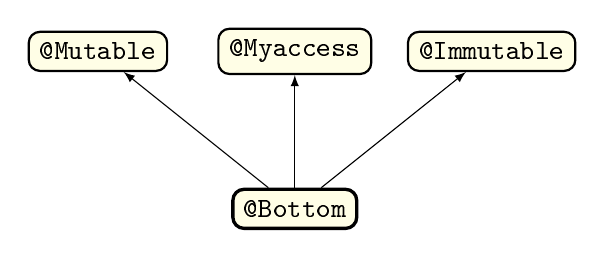
\begin{tikzpicture}[auto, >=latex]
      \tikzstyle{acc} = [draw, rectangle, fill=yellow!10, rounded corners, thick, inner sep=4pt]  
      \node [acc, very thick] (bot) at (0, 0) {\texttt{@Bottom}};
      \node [acc] (mut) at (-2.5, 2) {\texttt{@Mutable}};
      \node [acc] (mya) at (0, 2) {\texttt{@Myaccess}};
      \node [acc] (imm) at (2.5, 2) {\texttt{@Immutable}};
      
      \foreach \n in {mut,mya,imm} {
        \draw [->] (bot) -- (\n);
      }   
    \end{tikzpicture}
  }
  \tikzstyle{own} = [draw, rectangle, fill=green!10, rounded corners, thick, inner sep=4pt]    
  \subfigure[Ownership specifiers] {
    \begin{tikzpicture}
      \node [own] (safe) at (0, 0) {\texttt{@Safe}};
      \node [own] (anyo) at (-2, 2) {\texttt{@AnyOwner}}; 
      \node [own] (rep) at (0, 2) {\texttt{@Rep}};
      \node [own] (peer) at (2, 2) {\texttt{@Peer}};
      \node [own] (ondb) at (-3, 4) {\texttt{@OwnedBy}};
      \node [own] (world) at (-1, 4) {\texttt{@World}};
      
      \foreach \f/\t in {safe/anyo, safe/rep, safe/peer, anyo/ondb, anyo/world} {
        \draw [->] (\f) -- (\t);
      }
    \end{tikzpicture}  
  }
  \caption{Full hierarchy of type annotations defined in JimmuChecker}
  \label{fig:hierarchy}
\end{figure}

This section presents the type inference and verification rules used
by our checker. JimmuChecker works by~applying the type inference
rules to objects from user code and then checking the code against the
verification rules. Whenever a verification rule is violated,
the~checker signals an error. In the following discussion, annotated
types are written in~the~following form:

$$\underbrace{\mathtt{@A\quad @B}}_{\mathclap{\textrm{\small{type qualifiers}}}}\quad \overbrace{\mathtt{T}}^{\mathclap{\textrm{\small{Java type}}}}$$

\subsection{Subtyping}
\label{sec:chk:hierarchy}

JimmuChecker extends the functionality of the BaseTypeChecker
provided in the Checker Framework. BaseTypeChecker checks that if a
value of a type $S$ is assigned to~a~reference of~a~type $T$, then $S$
is a subtype of $T$. JimmuChecker makes use of this functionality,
which implies the following rule:

\setcounter{verrule}{-1}
\begin{verrule}[Subtyping]
  If a value of (annotated) type $S$ is assigned to a reference of type $T$, 
  then $S$ must be a subtype of $T$.
\end{verrule}
Figure \ref{fig:hierarchy} shows the hierarchy of type qualifiers used
in the checker. 

The \texttt{@Bottom} annotation exists for purely technical
reasons. In Checker Framework, each type must be annotated and
\texttt{@Bottom} serves the purpose of a default annotation where the~
\texttt{@Mutable} annotation is unsuitable. It is implicitly given to
constructs such as methods and classes, for which the concept of
(im)mutability makes no sense. The \texttt{@Bottom} annotation does
not need, and in fact should not, appear in user code.

Another important note is that each two \texttt{@OwnedBy} annotations
with different arguments are incomparable in the hierarchy, i.e. none
is a subtype of another.

There is a problem with the default subtyping mechanism in the Checker
Framework which has to be addressed here. BaseTypeChecker provides a
subtyping mechanism which would be~wrong for our
applications. Specifically, if $T$ had more than one type annotation
(e.g. \texttt{@A~@B~C}), it would be enough for $S$ to have an
annotation which subtypes \emph{one} of~the~annotations on the type
$T$ to be considered a subtype of $T$. This would lead to unwanted
results as, for~example, \texttt{@Immutable @Peer String} would
subtype \texttt{@Mutable @Safe String}, leading to~an~obvious
violation in~immutability when an \texttt{@Immutable} object gets
assigned to~a~\texttt{@Mutable} reference.

The class JimmuQualifierHierarchy is responsible for introducing
another mechanism of~subtyping. For each annotation $a$ on $T$ there
must be an annotation on $S$ which subtypes $a$. In~other words, each
annotation on the potential supertype is treated as a requirement
which has to be satisfied by the candidate subtype. 

It has to be emphasized that this rule applies not only to explicit
assignments, but is~also checked whenever an object is implicitly
assigned to a reference. This includes passing parameters to methods:
\begin{lstlisting}
Object copy(@AnyOwner Object z) { ... } 
// Cannot pass a @Rep value due to subtyping rule.
\end{lstlisting}
and invoking a method on an object: 
\begin{lstlisting}
public class C {
  Object z;
  Object copy() @OwnedBy(''z'') { ... } 
  // Cannot invoke on an object which is not owned by z
}
\end{lstlisting}

There are several exceptions to the subtyping rule which are
highlighted in the following subsections.

\subsection{Guarding immutability}

\subsubsection{Softening Rule 0}

The consequence of Rule 0 is that \texttt{@Mutable} objects cannot be
assigned to \texttt{@Immutable} re\-fe\-ren\-ces. This is in line with
Jimuva, whose authors state that allowing such \emph{upcasting} would
lead to an unsoundness within their type system. However, this seems
to be too strict for some real-life uses. Consider an instance method
of the \texttt{PeerStack} class (introduced in
Listing~\ref{lst:stack-peer} on page \pageref{lst:stack-peer}), whose
aim is to copy the structure of the stack. The method would be
declared in the following way:
\begin{lstlisting}
PeerStack copy(@Immutable PeerStack s) { ... }
\end{lstlisting}
to ensure that the original stack \texttt{s} remains unmodified. Rule
0, however, makes it impossible to call \texttt{copy} on a
\texttt{@Mutable} object, even though it would pose no danger to the
immutability properties. This observation is more general: any object
can be \emph{upcast} to a reference with stricter access restrictions,
i.e. \texttt{@Mutable} to~\texttt{@Myaccess} or \texttt{@Immutable}
and \texttt{@Myaccess} to~\texttt{@Immutable}, without violating
immutability.

To address the above discussion, JimmuChecker includes a mechanism
which allows users to~ease the restriction which Rule 0
carries. Whenever the \texttt{allow.upcast=true} option is~passed
to~the~checker, upcasting on access rights specifications is
permitted.

Effectively, the presence of the switch means that the checker has two
distinct modes of operation. The default behavior is compliant with
Jimuva in that it does not permit upcasting. Therefore, immutability
specifications on references (method parameters etc.) are to be
treated as requirements for the objects which are assigned to them,
i.e. only an~immutable object may be assigned to a variable annotated
with \texttt{@Immutable}. The modified behavior with
\texttt{allow.upcast} set to \texttt{true} is that \texttt{@Immutable}
is tied with an immutability contract on~the~reference rather than the
assigned object. An \texttt{@Immutable} annotation on~a~method
parameter, for example, means that the method may not modify the
object passed as~the~parameter.

\subsubsection{Enforcing \texttt{@ReadOnly} on methods} 
\label{sec:rules:readonly}

There are two aspects of enforcing the read-only property for methods.
Firstly, \texttt{@ReadOnly} methods must prevent the modification of
their receiver.

\begin{verrule}[Read-only method receivers] \label{vrl:readonly:rec}
  The receiver of a \texttt{@ReadOnly} method is implicitly marked
  with \texttt{@Immutable}. As an exception to Rule 0, access rights
  upcasting is allowed in this case, regardless of the
  \texttt{allow.upcast} option, so that \texttt{@ReadOnly} methods may
  be invoked on \texttt{@Mutable} objects.
\end{verrule}

Secondly, we must guard all values which are a part of an object's
internal representation from being modified inside a read-only
method. This is to avoid a situation where the state of an object
would be indirectly affected by a~call to a~read-only method
on~another object. Consider this example:

\begin{lstlisting}
  public class A {
    @Peer C value;
    @ReadOnly void foo() {
      value.modify(); 
    }
  }

  public class B {
    @Rep A a;
    @ReadOnly bar() {
      a.foo();
    }
  }
\end{lstlisting}

The method \texttt{bar()} should be considered correct as it calls a
read-only method. However, if it were not for the rule below, the
state of an object of class \texttt{B} could be indirectly modified 
by the method invocation \texttt{a.foo()}. 

\begin{verrule}[Indirect read-only
  protection] \label{vrl:readonly:meth} Encapsulated objects,
  i.e. those annotated with \texttt{@Peer} and \texttt{@OwnedBy}, are
  implicitly annotated with \texttt{@Immutable} inside read-only
  methods.
\end{verrule}

The above rule is an implementation of the read-only restriction of
Jimuva (\cite{haack}, page 10), albeit in an~eased form. We do not
forbid all field assignments, as mutable objects owned by~\emph{world}
may be modified without harm. Effectively, we enforce the same
restriction on~method invocations: only read-only methods may be
called on an object, unless it is owned by \emph{world}, in which case
there are no restrictions on method invocations.

\subsubsection{Guarding shallow state immutability} 

The following rule guards the shallow state immutability of immutable
objects:

\begin{verrule}[Shallow state immutability]
  If a value $w$ is \texttt{@Immutable}, its fields cannot be
  reassigned.
\end{verrule}
The following trivial code would therefore be illegal:
\begin{lstlisting}
public class IntHolder {
  public Integer n;
}

void test(@Immutable IntHolder h) {
  h.n = 0; /* Illegal */
}
\end{lstlisting}

\subsubsection{Resolving \texttt{@Myaccess}}  

Whenever an object containing \texttt{@Myaccess} elements is created
and used, the access rights variable is \emph{resolved}, depending on
the access rights on the object itself. This aims to protect the
immutability of \texttt{@Myaccess} elements of \texttt{@Immutable}
objects.

\begin{verrule}[Resolving \texttt{@Myaccess}]
  Elements annotated with \texttt{@Myaccess} are resolved in the
  following way:
  \begin{enumerate}[label=(\arabic*)]
  \item For a method call \texttt{x.m(\dots, @Myaccess z, \dots)}, the
    required access rights to \texttt{z} are the~same as~the~access
    rights to \texttt{x}.
  \item For a method call \texttt{x.m(\dots)}, if \texttt{x} returns a
    value annotated with \texttt{@Myaccess}, the access rights to the
    result are the same as the access rights to \texttt{x}.
  \item For a member select expression \texttt{x.f}, if \texttt{f} is
    annotated \texttt{@Myaccess}, the access rights to~the~whole
    expression are the same as the access rights to \texttt{x}.
  \end{enumerate}
\end{verrule}
Additionally, the \texttt{@Myaccess} annotation on any element within
an immutable class is immediately resolved to \texttt{@Immutable}.

Because \texttt{@Myaccess} can be resolved to \texttt{@Immutable}
using the above rule, values annotated with \texttt{@Myaccess} must be
protected from being modified inside read-only methods. The~protection
can be confined to read-only methods, because no other method may be
called on~an~immutable object, and \texttt{@Myaccess} only resolves to
\texttt{@Immutable} for immutable objects.

\begin{verrule}[\texttt{@Myaccess} protection]
  Inside read-only methods, if $v$ is a value annotated with
  \texttt{@Myaccess}:
  \begin{enumerate}
  \item non-read-only methods cannot be called on $v$, 
  \item fields of $v$ cannot appear in the left-hand side of an
    assignment.
  \end{enumerate}
\end{verrule}

\subsection{Enforcing constructor anonymity}
\label{sec:chk:anon}

Constructors of immutable objects should be annotated with
\texttt{@Anonymous}. JimmuChecker verifies that \texttt{@Anonymous}
constructors and methods do not leak references to \texttt{this},
which would allow foreign objects to observe the state of the object
being constructed, possibly before its state is fully
established. This would violate the property of immutability as stated
in Section \ref{sec:invariants}. 

To begin with, the checker has to have knowledge on which references
may point to~the~object under construction. We do not want, however,
to force the users to provide this information in their code. Instead,
JimmuChecker utilizes \emph{data-flow analysis} to infer information
on~dangerous references to \texttt{this}.

\subsubsection{Data-flow analysis in general} 

Generally, data-flow analysis is a static analysis technique used to
gather information on~what va\-lu\-es are possibly computed at a given
point of a program. The method consists in:
\begin{itemize}
\item modifying the information available in the pre-state of each
  statement to~obtain the~information in the post-state, according
  to~the~form of~the~statement, 
\item branching and merging the information on conditional statements,
  loops etc.
\end{itemize}
Data-flow analysis may be used, for example, to compute the reach of
particular variable definitions in a program, the set of \emph{live}
variables which contribute to the overall result, and~many more
program properties. A comprehensive introduction to data-flow analysis
can be found in~\cite{dataflow}. 

\subsubsection{Inferring information on references to \texttt{this}} 

In JimmuChecker, a simple inter-procedural data-flow analysis is
performed prior to verification using an implementation supplied in
the Checker Framework, with the class \texttt{JimmuFlow} responsible
for the analysis. It aims to annotate expressions with one of three
possible annotations: \texttt{@This}, \texttt{@MaybeThis} and
\texttt{@NotThis}. The annotations are internal for JimmuChecker: they
should not appear in user code, but may show up in error messages
printed by~the~checker.

The analyzer stores a map from element (variable, parameter etc.)
identifiers into the relevant annotation for each place in code.
Below, we present a simplified set of typing rules for expressions
which are applied during the flow analysis. As usual in type systems,
$x : \tau$ denotes that the value $x$ is of type $\tau$. Moreover, $x
: \lbrace\tau_1, \tau_2\rbrace$ is be used as an abbreviation for the
alternative $x : \tau_1 \lor x : \tau_2$.

Note that the rules below are only valid if we assume that the
verification rule for anonymity, which is presented as
Rule~\ref{vrl:anon} in the following subsection, holds for all
anonymous methods. In this sense, the verification and inference rules
are intertwined: the verification rule uses the inferred types and the
inference rules assume the verification rule.

\def\proofSkipAmount{\vskip 0.4cm}
\begin{prooftree}
  \AxiomC{}
  \RightLabel{(this)}
  \UnaryInfC{$\mathtt{this} : \texttt{@This}$}
\end{prooftree}

\begin{prooftree}
  \AxiomC{}
  \RightLabel{(new)}
  \UnaryInfC{\texttt{new} C($\vec{p}$) : \texttt{@NotThis}}
\end{prooftree}

\begin{prooftree}
  \AxiomC{x : $\lbrace \mathtt{@This}, \mathtt{@MaybeThis}\rbrace$}
  \RightLabel{(this-member)}
  \UnaryInfC{x.f : \texttt{@MaybeThis}}
\end{prooftree}

In the following rules, (nthis-member) and (nthis-inv), we assume that
a reference to \texttt{this} has not been leaked to another
object. This means that the enforcing of the \texttt{@Anonymous}
annotation is not absolute. A call to an anonymous method might, in
fact, unwittingly leak \texttt{this} references if the object has
already leaked such a reference and passed it back to~the~anonymous
method or assigned to a field. Notice, however, that this does
not~harm the~immutability properties, because anonymity is only
crucial during construction.

\begin{prooftree}
  \AxiomC{x : \texttt{@NotThis}}
  \RightLabel{(nthis-member)}
  \UnaryInfC{x.f : \texttt{@NotThis}}
\end{prooftree}

\begin{prooftree}
  \AxiomC{x : \texttt{@NotThis}}
  \RightLabel{(nthis-inv)}
  \UnaryInfC{x.m($\vec{p}$) : \texttt{@NotThis}}
\end{prooftree}

The next rule, (anon-this-inv), is a direct consequence of
point~\ref{pnt:anon-ret} of Rule \ref{vrl:anon}.

\begin{prooftree}
  \AxiomC{m : \texttt{@Anonymous}}
  \AxiomC{x : $\lbrace \mathtt{@This}, \mathtt{@MaybeThis}\rbrace$}
  \RightLabel{(anon-this-inv)}
  \BinaryInfC{x.m($\vec{p}$) : \texttt{@NotThis}}
\end{prooftree}

\begin{prooftree}
  \AxiomC{$\neg$ (m : \texttt{@Anonymous})}
  \AxiomC{x : $\lbrace \mathtt{@This}, \mathtt{@MaybeThis}\rbrace$}
  \RightLabel{(nanon-this-inv)}
  \BinaryInfC{x.m($\vec{p}$) : \texttt{@MaybeThis}}
\end{prooftree}

\begin{prooftree}
  \AxiomC{$p$ is a parameter of a constructor}
  \RightLabel{(param-ctor)}
  \UnaryInfC{p : \texttt{@NotThis}}
\end{prooftree}

The final rule, (param-meth), takes a conservative approach by taking
into consideration situations when the user might pass a reference to
\texttt{this} as an argument to~its~own instance method.

\begin{prooftree}
  \AxiomC{$p$ is a parameter of a method}
  \RightLabel{(param-meth)}
  \UnaryInfC{p : \texttt{@MaybeThis}}
\end{prooftree}

The types inferred using the above rules are subsequently propagated
along with the~va\-lu\-es. Whenever a value appears in the user's
code, JimmuChecker recalls the annotations on~the~previous
appearances. When considering branching statements, such as the
conditional branch \texttt{if} and the \texttt{while}-loop,
JimmuChecker takes a conservative approach, possibly coming up with
spurious errors, but ensuring that the immutability property
holds. The propagation rules which handle branching operations utilize
a relation $\cup$ which is defined as~shown in~Table~\ref{tbl:cup}.
\begin{table}[h]
  \centering
  \begin{tabular}{c|c|c|c|}
    $\cup$ & \texttt{@This} & \texttt{@MaybeThis} & \texttt{@NotThis} \\ \hline
    \texttt{@This} & \texttt{@This} & \texttt{@MaybeThis} & \texttt{@MaybeThis} \\ \hline
    \texttt{@MaybeThis} & \texttt{@MaybeThis} & \texttt{@MaybeThis} & \texttt{@MaybeThis} \\ \hline
    \texttt{@NotThis} & \texttt{@MaybeThis} & \texttt{@MaybeThis} & \texttt{@NotThis} \\ \hline
  \end{tabular}
  \caption{The $\cup$ relation}
  \label{tbl:cup}
\end{table}

Propagation rules are rules which decide how annotations on elements
change between instructions. The expression typing rules presented
above introduce a mapping from code elements (variables, method
parameters etc.) into the set $\lbrace$\texttt{@This},
\texttt{@MaybeThis}, \texttt{@NotThis}$\rbrace$ of annotations. This
mapping may be then modified by program statements, as per
the~propagation rules.

Several example propagation rules are shown below in Hoare
logic~\cite{hoare}. The simplest rules are the ones related to
assignment.

\begin{prooftree}
  \AxiomC{v : $\tau$} 
  \RightLabel{(assign)} 
  \UnaryInfC{\htr{true}{x = val}{x : $\tau$}}
\end{prooftree}

\begin{prooftree}
  \AxiomC{}
  \RightLabel{(alias)}
  \UnaryInfC{\htr{var : $\tau$}{x = var}{x : $\tau$}}
\end{prooftree}

In the following rules, $\phi$ stands for an undisclosed thesis
regarding the mapping of variables to types which is valid in the
pre-state of the analyzed statement. 

When subsequently executing two statements, we propagate the theses
($\psi$) resulting from the post-state of the first statement to the
pre-state of the second one:

\begin{prooftree}
  \AxiomC{\htr{$\phi$}{$P_1$}{$\psi$}}
  \AxiomC{\htr{$\psi$}{$P_2$}{x : $\tau_2$}}
  \RightLabel{(semicolon)}
  \BinaryInfC{\htr{$\phi$}{\texttt{$P_1$; $P_2$}}{x : $\tau_2$}}
\end{prooftree}

Conditional statements conserve annotations from all branches using
the $\cup$ operator:

\begin{prooftree}
  \AxiomC{\htr{$\phi$}{$P_1$}{x : $\tau_1$}}
  \AxiomC{\htr{$\phi$}{$P_2$}{x : $\tau_2$}}
  \RightLabel{(if)}
  \BinaryInfC{\htr{$\phi$}{\texttt{if (}$C$\texttt{)} $P_1$ \texttt{else} $P_2$}{x : $\tau_1 \cup \tau_2$}}
\end{prooftree}

\begin{prooftree}
  \AxiomC{$\phi \to x : \tau_1$}
  \AxiomC{\htr{$\phi$}{$P$}{x : $\tau_2$}}
  \RightLabel{(while)}
  \BinaryInfC{\htr{$\phi$}{\texttt{while (}$C$\texttt{)} $P$}{x : $\tau_1 \cup \tau_2$}}
\end{prooftree}

\begin{prooftree}
  \AxiomC{\htr{$\phi$}{$P_1$}{x : $\tau_1$}}
  \AxiomC{\htr{$\phi$}{$P_2$}{x : $\tau_2$}}
  \AxiomC{\htr{$\phi$}{$P_3$}{x : $\tau_3$}}
  \RightLabel{(try-catch-finally)}
  \TrinaryInfC{\htr{$\phi$}{\texttt{try} $P_1$
      \texttt{catch(}e\texttt{)} $P_2$ \texttt{finally} $P_3$}{x :
      $\tau_1 \cup \tau_2 \cup \tau_3$}}
\end{prooftree}

Let us consider an example process of inferring the annotations. The
following code is to~be~checked, which is a part of an implementation
of a singly-linked list of integers delimited by a node whose
\texttt{next} pointer references the node itself.
\begin{lstlisting}
class IntList {
  Integer value;
  IntList next;

  public IntHolder(Integer n, IntList nxt) {
    this.value = n;
    if (nxt == null) {
      this.next = this;
    } else {
      this.next = nxt;
    }
    initialize(this.next);
  }
\end{lstlisting}
Let us assume that the method \texttt{initialize} called here is not
annotated with \texttt{@Anonymous}. By the expression typing rules,
the following mapping of variables to types are valid at the beginning
of the method:
\begin{itemize}
\item \texttt{n} : \texttt{@NotThis} by (param-ctor)
\item \texttt{nxt} : \texttt{@NotThis} by (param-ctor)
\item \texttt{value} : \texttt{@MaybeThis} by (this-member)
\item \texttt{next} : \texttt{@MaybeThis} by (this-member)
\end{itemize}
In the post-state of the first assignment, \texttt{this.value = n},
the type of \texttt{value} is changed to~\texttt{@NotThis} by the
(alias) rule. Next, we analyze the conditional statement. The first
branch assigns a value of type \texttt{@This} to the \texttt{next}
field of the constructed object, while the other branch assigns a
\texttt{@NotThis}. The (if) rule is now used to merge the two
branches. The result is that the two types are combined using the
$\cup$ operator into the \texttt{@MaybeThis} type, which becomes the
type of the field in the post-state of the conditional statement.
Therefore, the~method invocation in the last statement of the method
is an error by Rule~\ref{vrl:anon}.

\subsubsection{Rules for anonymity} 

Having introduced the concept and mechanism of tracing references to
\texttt{this} inside constructors, we can finally state the rules
related to anonymity which are verified by JimmuChecker.

\begin{verrule}[Anonymity] \label{vrl:anon}
  Whenever a method \texttt{m} is annotated \texttt{@Anonymous}, if
  $x$ is a value of type \texttt{@This} or \texttt{@MaybeThis}:
  \begin{enumerate}[label=(\arabic*)]
  \item \label{pnt:anon-ret} \texttt{m} cannot return $x$, 
  \item \texttt{m} cannot call non-anonymous methods on $x$, 
  \item inside \texttt{m}, $x$ cannot be passed as an argument to a constructor, 
  \item inside \texttt{m}, $x$ cannot be passed as an argument to a
    method of a foreign object (of type \texttt{@NotThis} or
    \texttt{@MaybeThis}),
  \item inside \texttt{m}, $x$ cannot be assigned to an object field
    or an array field.
  \end{enumerate}
\end{verrule}

The above rule makes it impossible for a checked \texttt{@Anonymous}
method to leak references to \texttt{this}, provided that such a
reference has not already been leaked.

In order to protect the first immutability property, we have to ensure
that a reference to \texttt{this} does not leak while an immutable
object is constructed. Therefore, JimmuChecker issues a warning
whenever the following rule is violated:
\begin{verrule}[Anonymous construction of immutable objects]
  Every immutable object must be constructed using an anonymous
  constructor.
\end{verrule}


\subsection{Encapsulation of representation}
\label{sec:chk:rep}

Enforcing encapsulation of representation aims to guard the deep
internal state of immutable objects from being modified. As discussed
in Section~\ref{sec:mod:ownership}, the internal state of object $w$
consists of~all objects which are owned by $w$, whether directly -- by
assigning them to a \texttt{@Rep}-annotated reference or by using the
\texttt{@OwnedBy} annotation -- or indirectly -- through the
\texttt{@Peer} annotation on a member of an object already owned by
$w$.

\subsubsection{Encapsulation property} 

Encapsulation of representation not only protects the deep state of
immutable objects from modifications, but also prohibits access to
internal objects from the outside. This results in~a~situation when
the internal state of $w$ is only accessible through $w$'s interface,
except from when $w$ decides to entrust another object with a
reference to an object it owns by passing it~as~a~(\texttt{@Safe})
parameter to a method. Even considering this exception, JimmuChecker
ensures that, in addition to the invariants defined in
Section~\ref{sec:invariants}, the following property is~satisfied in
all checked code:

\begin{invariant}[Encapsulation of representation] \label{inv:encap}
  If $v$ is a part of~the state of an object $w$, then no mutable
  static aliases are created to $v$ or~any part of~$v$'s state outside
  $w$'s state as a consequence of actions of objects in $w$'s state.
\end{invariant}

Of course, such static references to $v$ may have existed prior to
being passed to the inside of $w$'s state. The following example
ilustrates the situation:

\begin{lstlisting}
public class A {
  private @Rep Object o;
  public void set(@Rep Object o) {
    this.o = o;
  }
}

void initA(A a) {
  Object ao = new @OwnedBy(''a'') Object();
  ...
  a.set(ao);
}
\end{lstlisting}

We cannot prohibit the method \texttt{initA} from sharing the object
\texttt{ao} with other objects before or after it is passed to its
owner \texttt{a}. What we ensure with Property~\ref{inv:encap} is that
\texttt{a} itself does not leak the reference to its internal
representation object \texttt{a.o} to the outside.

The rest of this section details on how the above invariant, and the
immutability invariant with regards to deep state of objects, are
enforced.

\subsubsection{Guarding encapsulation and deep state immutability} 

The following rules are enforced by JimmuChecker in order to guard
internal state encapsulation and the immutability property with
regards to the deep state of objects.

\begin{verrule}[Encapsulation of representation]
  If $v$ is a value annotated with \texttt{@Rep}:
  \begin{enumerate}[label=(\arabic*)]
  \item a non-immutable reference to $v$ cannot be returned from
    methods.
  \item $v$ cannot be passed as a non-immutable and non-safe parameter
    to methods of fo\-reign objects which are not annotated with
    \texttt{@Rep}. Foreign objects are objects which are not marked
    with the \texttt{@NotThis} annotation by the data-flow analysis
    described in~Section~\ref{sec:chk:anon}
  \item $v$ cannot be passed as a non-immutable and non-safe parameter
    to constructors, unless the constructor creates an object whose
    ownership specification is \texttt{@Rep}.
  \item $v$ cannot be declared \texttt{public}. 
  \end{enumerate}
  Moreover, if $w$ is an object with a \texttt{@Rep}-annotated member
  $v$,
  \begin{enumerate}[label=(\arabic*), resume]
  \item $v$ cannot be directly accessed by other objects, i.e. the
    expression \texttt{w.v} is erroneous, even if Java visibility
    mechanism would permit such access.
  \end{enumerate}
  If $v$ is annotated with \texttt{@Peer}:
  \begin{enumerate}[label=(\arabic*), resume]
  \item $v$ cannot be passed as a non-immutable and non-safe parameter
    to methods of foreign objects which are not annotated with
    \texttt{@Rep} or \texttt{@Peer}.
  \item $v$ cannot be passed as a non-immutable and non-safe parameter
    to constructors, unless the constructor creates an object whose
    ownership specification is \texttt{@Rep} or \texttt{@Peer}.
  \end{enumerate}
\end{verrule}

Note that an object may freely share with the outside world the
immutable references to~its~internal representation. This is in line
with Jimuva (cf. the Sub Share subtyping rule of the type system on
page 12 of~\cite{haack}) and other ownership systems described in
Section~\ref{sec:rel:ownership}. Naturally, this does not violate
immutability invariants as the passed references cannot be~used to
modify the representation. 

\begin{verrule}[Deep state immutability] \label{vrl:deepimm}
  If $w$ is an immutable object holding a \texttt{@Rep}-annotated
  reference to $v$, then:
  \begin{enumerate}[label=(\arabic*)]
  \item only read-only methods may be called on $v$, 
  \item $v$ may not be passed as a non-immutable argument to a method
    or constructor.
  \item no field of $v$ can be reassigned, i.e. any assignment of the
    form \texttt{v.f~=~x}, is illegal.
  \item \label{pnt:deep-array} if $v$ is an array, no element of $v$
    can be reassigned, i.e. any assignment of the form
    \texttt{v[i]~=~x}, is illegal,
  \end{enumerate}
\end{verrule}
Note that Rule \ref{vrl:deepimm} also applies to the receivers of
read-only methods, which are implicitly immutable by
Rule~\ref{vrl:readonly:rec}. 

In point \ref{pnt:deep-array} of the rule, if the fields of the
array $v$ are arrays declared as members of $w$'s state with the
syntax like
\begin{center}
  \texttt{protected Object @Rep [] @Rep [];}
\end{center}
then the fields of the arrays also cannot be reassigned. This applies
to deeper levels of array nesting as well. 

\subsubsection{Checking \texttt{@OwnedBy} argument validity} 

Whenever a variable, field or parameter is annotated with
\texttt{@OwnedBy}, JimmuChecker verifies that the annotation's
argument matches a reference which exists in the annotated object's
scope. The argument is expected to be a Java string containing a
single identifier or a non-empty chain of identifiers (of the form
$x_1.x_2.\cdots.x_n$). The first identifier in the chain refers to the
\emph{base} object or class, which must be in the annotated object's
scope, whilst the other identifiers describe the path to an object
reachable from the base through public fields.

$$ \mathtt{@OwnedBy("}\underbrace{\mathtt{list}}_{\mathclap{\textrm{base}}} 
\mathtt{.}
\underbrace{\mathtt{next.next}}_{\mathclap{\textrm{member path}}}\mathtt{")} $$

Objects of the class \texttt{JimmuVisitor.Owner} represent the
owners. The class' constructors parse the arguments of
\texttt{@OwnedBy} annotations and signal any errors found therein.

The constructors first search the current scope for an element with a
name equal to~the~base. To this end, the \texttt{JimmuVisitorState}
stores a stack representing blocks with declared variables. This
stack, along with the methods and classes enclosing the place of code
being inspected, is~scanned for a matching element. If such an element
is found, the algorithm proceeds to~scan the class whose instance the
base is, as well as its superclasses, for a member matching the~first
element of the patch. The process continues with the class of this
path element and the next element.

An important feature here is that \texttt{Owner} objects store the
annotated types of the owner objects. This enables the checker to
identify objects whose owners are immutable or annotated with
\texttt{@Myaccess}, which is crucial for the rules described in the
next paragraph.

\subsubsection{Inferring access rights on \texttt{@OwnedBy} references} 

According to the definition of object state on page
\pageref{def:state}, objects annotated with \texttt{@OwnedBy(''z'')}
are part of the state of \texttt{z}. Therefore, in order to satisfy
the immutability properties, we must ensure that objects which are
owned by immutable objects are also immutable. This is done by
inferring access rights on owned objects which are the same or
stricter as the access rights of the owner object:

\begin{verrule}[Access rights of \texttt{@OwnedBy} objects]
  If an object $x$ is annotated with \texttt{@OwnedBy(''z'')} and
  \texttt{z} refers to an immutable object, the~access rights of $x$
  are implicitly changed to \texttt{@Immutable}. Analogously, if
  \texttt{z} refers to an object annotated with \texttt{@Myaccess},
  the access rights of $x$ are changed to \texttt{@Myaccess} provided
  that $x$ is not already annotated with \texttt{@Immutable}.
\end{verrule}
\vspace{-0.7cm}

\subsubsection{Resolving ownership} 

One of the main inherent differences between Jimuva and our checker is
that Java annotations specifying ownership are \emph{relative}: we may
refer to the same object with different ownership specifications,
depending on the place of code where the owned object is declared. As
a result, to~understand which object is actually the owner, one must
know the annotation and the place of~code where the annotated
reference is declared.

Let us consider an example. The class \texttt{IntList} is meant to
implement a simple singly-linked list of integers, with the integer
belonging to the internal representation of a relevant cell. 
\begin{lstlisting}
public class IntList {
  private @Rep Integer n;
  private IntList l;

  public IntList(Integer n, IntList l) {
    this.n = new @Rep Integer(n);
    this.l = l;
  }

  public changeHead(@Rep Integer newN) {
    this.n = newN;
  }
}

public class Test {
  public static void test() {
    IntList l = new IntList(1, null);
    @Rep nh = new @Rep Integer(0);
    l.changeHead(nh); /* Wrong! */
  }
}
\end{lstlisting}
In the \texttt{test()} method, allowing the invocation of
\texttt{l.changeHead} would be wrong, even though the \texttt{@Rep}
annotation matches on both the actual argument \texttt{nh} and the
formal parameter of~the~method. The owners of the two objects are
different: \texttt{nh} is owned by the instance of~\texttt{Test} while
the parameter \texttt{newN} of method \texttt{l.changeHead} is
supposed to be owned by~the~list head \texttt{l}. The correct way to
invoke the method would be:
\begin{lstlisting}
@OwnedBy(''l'') nh = new @OwnedBy(''l'') Integer(0);
l.changeHead(nh); /* Correct! */
\end{lstlisting}

The above discussion leads to the concept of \emph{ownership
  resolving}. It is a process of changing the relative ownership
specifications on elements so that they reflect the true ownership
relations. Ownership resolving must take place whenever two objects
interact, namely on:
\begin{itemize}
\item member access, i.e. expressions such as \texttt{x.y},
\item returning a value from a method, 
\item passing parameters to a method or constructor.
\end{itemize}
Of course, the subtyping rule (Rule 0) acts upon the modified
(resolved) ownership specifications.

In the first two cases, we have two non-trivial possibilities to
handle: if the returned value or the field is annotated with
\texttt{@Peer} and \texttt{@OwnedBy}. The \texttt{@World} annotation
remains unchanged and \texttt{@Rep} values cannot be returned from
methods or directly accessed at all.

\begin{verrule}[Resolving ownership: member access and return values]
  \label{vrl:res:acc}
  If the expression $x$ evaluates to a reference annotated with
  the ownership specification $T$, then:
  \begin{enumerate}[label=(\arabic*)]
  \item if $v$ is a field of $x$ annotated with \texttt{@Peer}, then
    the ownership of the expression \texttt{x.v} is~resolved to $T$;
  \item \label{pnt:peer-ret} if the method \texttt{m} has a return value which is annotated
    with \texttt{@Peer}, then the~ownership of the expression
    \texttt{x.m($\vec{p}$)} is resolved to $T$.
  \end{enumerate}
  If $x$ is a reference, or a chain of identifiers (such as
  \texttt{l.next.next}) which evaluates to an object reference, then
  \begin{enumerate}[label=(\arabic*), resume]
  \item if $v$ is a field of $x$ annotated with
    \texttt{@OwnedBy(''z'')}, then the ownership of the expression
    \texttt{x.v} is resolved to @OwnedBy(''x.z'');
  \item if the method \texttt{m} has a return value which is
    annotated with \texttt{@OwnedBy(''z'')}, then the~ownership of
    the expression \texttt{x.m($\vec{p}$)} is resolved to
    \texttt{@OwnedBy(''x.z'')}.
  \end{enumerate}
\end{verrule}

Argument passing is slightly more sophisticated as a method may have a
formal argument annotated with \texttt{@Rep}, and this additional case
must be handled as well. The rule below is~enacted by~changing the
expected annotated type of an actual argument of a method whenever the
method is invoked. The expected argument type is changed depending
on~the~ownership specifications of the formal parameter of the method,
and of the object on which the method is invoked.

\begin{verrule}[Resolving ownership: passing arguments to methods]
  If $x$ is a reference, or a chain of identifiers evaluating to a
  reference, with an ownership specification $T$, and $x$ has an
  instance method \texttt{m}, then for each formal parameter $p_i$ of
  $m$, the~actual parameter passed into the method via the invocation
  \texttt{x.m($\vec{p}$)} is expected to have an ownership
  specification $T_{p_i}$ as follows:
  \begin{enumerate}[label=(\arabic*)]
  \item if $p_i$ is annotated with \texttt{@Rep}, $T_{p_i}$ is
    \texttt{@OwnedBy(''x'')};
  \item if $p_i$ is annotated with \texttt{@Peer}, $T_{p_i} = T$;
  \item if $p_i$ is annotated with \texttt{@OwnedBy(''z'')}, $T_{p_i}$
    is \texttt{@OwnedBy(''x.z'')}.
  \end{enumerate}
\end{verrule}

Since the ``receiver'' of a constructor does not exist before the
constructor is called, it makes no sense to annotate constructor
arguments with \texttt{@Rep}. Also, \texttt{@OwnedBy} specifications
may only refer to outside objects and not the constructed object's
fields. Therefore, the ownership resolving rule for constructors is
simpler:

\begin{verrule}[Resolving ownership: passing arguments to constructors]
  Whenever a constructor is called to create an object with an
  ownership specification $T$, for~each formal parameter $p$ of the
  constructor, the actual parameter passed into the constructor
  is~expected to have an ownership specification $T_p$ as follows:
  \begin{enumerate}[label=(\arabic*)]
  \item if $p$ is annotated with \texttt{@Peer}, $T_p = T$;
  \item if $p$ is annotated with \texttt{@OwnedBy(''z'')}, $T_p$ is
    unchanged.
  \end{enumerate}
\end{verrule}

For an example on ownership resolving, please consider the class
\texttt{PeerStack} defined on~page~\pageref{lst:stack-peer}. Inside
the \texttt{pop()} method, the \texttt{result} variable is annotated
with \texttt{@Peer} and~is~assigned a value returned from
\texttt{head.getData()}. The assignment is correct by point
\ref{pnt:peer-ret} of~Rule~\ref{vrl:res:acc}, because
\texttt{getData()} returns a \texttt{@Peer} value, and \texttt{head}
is itself annotated with~\texttt{@Peer}.

\subsection{Enforcing the safety of \texttt{@Safe} values}
\label{sec:chk:safe}

\texttt{@Safe} method parameters are a way of adapting Jimuva's
concept of owner-polymorphic methods for our checker. Encapsulated
values -- annotated with \texttt{@Peer} or \texttt{@Rep} -- may
be~passed as~safe parameters to methods. Therefore, elements annotated
by \texttt{@Safe} should be protected in a special way in order to
satisfy the encapsulation property specified on
page~\pageref{inv:encap}. Namely, no static aliases may be created to
safe values.

This condition is partially enforced by the subtyping rule itself: as
shown in Figure~\ref{fig:hierarchy}, \texttt{@Safe} is the supertype
of all ownership specifications. The subtyping mechanism implemented
in JimmuChecker thus ensures that a safe value is never assigned to a
non-safe value. However, checked code may also call unchecked
methods. In that case, the subtyping rule would be~of~no~use, as there
would be no ``requirements'' present on the method parameters, which
would lead to safe values being passed freely to unchecked code.

The following rules must be enforced to ensure that no static aliases
are created to safe values:

\begin{verrule}[Direct safety]
  A safe value may never be assigned to fields. 
\end{verrule}
\vspace{-0.8cm}
\begin{verrule}[Indirect safety]
  \begin{enumerate}[label=(\arabic*)]
  \item A safe value may never be passed as a non-safe parameter to a
    method.
  \item A method whose receiver is not annotated with \texttt{@Safe}
    may not be called on a safe object.
  \end{enumerate}
\end{verrule}

When an object is safe, we should protect from static aliasing not
only the object itself, but also its transitive reach.  Consider the
following example. Again, it uses a~\texttt{PeerStack}
(page~\pageref{lst:stack-peer}), but imagine that the class'
\texttt{head} field and the \texttt{Cell<T>} class are~public:
\begin{lstlisting}
  public class StackViolator<T> {
    private Cell<T> f;
    void violate(@Safe PeerStack<T> s) {
      f = s.head;
    }
  }
\end{lstlisting}
If it were only for the above safety rules, the assignment would
type check and produce a~static alias to an object which is owned by
the owner of \texttt{s} and should be encapsulated. The violation
stems from the fact that \texttt{s.head} is not protected in any way.

The rule below completes the rules necessary to protect the safety of
values. Note that only \texttt{@Peer} objects must be protected
because \texttt{@Rep} objects are not accessible through return values
and member access.
\begin{verrule}[Transitive reach safety]
  If \texttt{x} is a safe value, and:
  \begin{enumerate}[label=(\arabic*)]
  \item if \texttt{f} is a \texttt{@Peer} field of \texttt{x}, the
    expression \texttt{x.f} is also safe, 
  \item if a method \texttt{m} of \texttt{x} returns a \texttt{@Peer}
    value, the expression \texttt{x.m($\vec{p}$)} is also safe. 
  \end{enumerate}
\end{verrule}

\subsection{Handling immutable classes}

Immutable classes (annotated with \texttt{@ImmutableClass}) have a
special place in JimmuChecker's type system. Instances of immutable
classes are the objects that satisfy the crucial property --
immutability in an open world -- defined on
page~\pageref{inv:open}. Therefore, immutable classes should contain
some additional means of protection so that their state may not be
mutated by~unchecked code.

There are several dangers to the open-world immutability
here. Firstly, immutable classes may be instantiated with any
constructor they define, so no constructor should be allowed to leak a
reference to the object being constructed. Secondly, no checking is
performed for~method calls from unchecked code. Therefore, all methods
must be read-only to prevent modification of the object's
state. Thirdly, if an immutable class has a non-final public field,
the field may be accessed and reassigned by unchecked code. Note that
in the latter case, protected fields are not a problem, as we assume
that immutable classes are not illegally subclassed, i.e. all their
subclasses are also immutable.

In order to protect the immutability of the instances, the following
rule must be applied:
\begin{verrule}[Immutable classes]
  If $C$ is an immutable class, 
  \begin{enumerate}[label=(\arabic*)]
  \item all constructors of $C$ are implicitly annotated with \texttt{@Anonymous},
  \item all methods of $C$ are implicitly annotated with \texttt{@ReadOnly},  
  \item all fields of $C$ must be \texttt{protected}, \texttt{private} or \texttt{final}.
  \end{enumerate}
\end{verrule}

Whenever a violation occurs inside a method or constructor which is
implicitly annotated, the error message printed by JimmuChecker 
contains a relevant note, so that the user is~not~confused that the
checker verifies an annotation which is not present in their code.

We also have to protect immutable classes from being illegally
subclassed: 
\begin{verrule}
  The \texttt{@ImmutableClass} annotation is inherited, i.e. each
  (checked) subclass of an immutable class is also immutable. 
\end{verrule}

Let us complete the set of rules with a self-explanatory rule which
applies to checked code:
\begin{verrule}[Immutable class instancing]
  Any object of an immutable class must be immutable. 
\end{verrule}

\section{Conclusions}

JimmuChecker is a complete tool for verifying object immutability, as
well as class immutability in an open world. As a compiler plug-in,
the checker is easy to use and may be smoothly integrated into the
normal development process of any Java system. It can help avoid
and~fight common errors related to object immutability. On the other
hand, the type system used by~JimmuChecker is elastic enough to allow
for implementing design patterns such as iterators: the source code
for the checker is accompanied by a relevant example.

\subsection{Future work}

JimmuChecker still does not cover some of the more sophisticated
constructs of Java. Among the possible extensions are:
\begin{itemize}
\item Allowing the static fields of any class to be owners of objects
  through the use of reflection, 
\item Introducing immutable class support into Java's reflection
  mechanism. The~checker is~currently oblivious to the fact that a
  class is an \texttt{@ImmutableClass} if the class is~loaded
  dynamically via reflection.
\end{itemize}

The checker can also be extended into another area, which is related
to object immutability: method purity and determinism. 

A method should be considered \emph{pure} if it does not modify the
state of any object, and~a~class would be called \emph{pure} if it is
immutable and all methods are pure. There are several approaches to
verifying method purity. For the purpose of extending JimmuChecker
with a purity checker, the most suitable one seems to be the modular
type system JPure \cite{jpure}.

A method should be considered \emph{deterministic} if its result is
the same whenever it is called with the same arguments (the receiver
being treated as an additional argument). It is apparent here that the
concept of ownership would play an important role here, as it would
help define what it means that method arguments are the same by
introducing the deep state of objects. 

The only approach to verifying the determinism of Java methods we are
aware of has been created within Joe-E \cite{deterministic}. Joe-E
itself is a subset of Java which strictly adheres to~the~rules
of~the~object-capability model described above. The verification of
method determinism introduces shallow-state immutability through the
use of the \texttt{final} modifier and a~method is~considered
deterministic if all its arguments, including the receiver, are
immutable. While this, along with the properties of the
object-capability model, does guarantee method determinism, this seems
to be too strict. Another approach, relying on deep states to compare
objects, could be taken to verify whether Java methods are
deterministic.

\chapter{Related work}
\label{chap:related}

In this chapter, we recall some of the previous attempts at creating
type systems for~ve\-ri\-fi\-ca\-tion of~object ownership and
immutability, and at implementing relevant checkers. We also reflect
on how those approaches relate to our work.

\section{Ownership type systems}
\label{sec:rel:ownership}

Ownership type systems have been a matter of interest for researchers
for over a decade now. The main issue which has to be tackled has
already been mentioned in this work: simultaneously maintaining
sufficient expressiveness of the language and the necessary
encapsulation of internal representation of objects. 

\subsection{Boyapati et al.'s ownership types}

Boyapati et al.~\cite{own-encap} introduced an ownership type system
for a Java-like language obtained by~extending object types with
ownership specifications. Their explicit ownership variables are
limited to \texttt{this} and \texttt{world} (apart from those,
\texttt{peer} and any object identifier may be~used
in~Jimuva). However, their language is expressive enough -- it may for
example express iterators -- because of the owner-polymorphism which
allows for more than one ownership parameters for classes and
methods. Let us look at an implementation skeleton of a stack holding
values of type \texttt{T}.

\begin{lstlisting}
class TStack<stackOwner, TOwner> {
  TNode<this, TOwner> head;
  ...
}

class TNode<nodeOwner, TOwner> {
  TNode<nodeOwner, TOwner> next;
  T<TOwner> value; 
}
\end{lstlisting}

The classes are parameterized not only with their own ownership (via
the \texttt{stackOwner} and~\texttt{nodeOwner} variables), but also
with the variable \texttt{TOwner} representing the owner of~the~stack
elements. This allows the class to be instantiated in multiple ways:
\begin{lstlisting}
class TStackClient<clientOwner> {
  TStack<this, this> s1 = new TStack<this, this>();
  TStack<this, world> s2 = new TStack<this, world>();
  TStack<world, world> s3 = new TStack<world, world>();
}
\end{lstlisting}
which would require the \texttt{@Peer} annotation in our type system. 

\subsection{Universes}

A different approach has been taken by Dietl and Müller in their
Universes type system~\cite{universes}. The general idea behind their
work was to organize objects into \emph{contexts} or \emph{ownership
  domains} which share the same owner. This is done by employing the
two keywords which are also used in JimmuChecker: \texttt{rep} to
denote an object owned by the referencing object and \texttt{peer} to
denote an object within the same context as the referencing
object. Owner-as-modifier encapsulation is enforced by ensuring that
there no read-write references to an object are present outside of the
context the object belongs in. Read-only references, on the other
hand, may be freely shared with the outside world.

\subsection{ArchJava}

In Universes, a single ownership domain is bound to every object. This
was considered to~be~an~important limitation by Aldrich and
Chambers~\cite{domains}, who developed an ownership type system used
in the ArchJava system for enforcing the proper architectural
structure for~Java programs~\cite{archjava}. The ownership type system
allows the user to specify multiple ownership domains for one
object. To overcome the restrictions imposed by encapsulation
of~representation, ownership domains can be \emph{linked} so that one
can access the other across domain boundaries.

Both Universes (in its revised version cited here) and ArchJava are
expressive enough to allow implementing iterators and~other important
design patterns.

\section{Javari: reference immutability}

The Javari language and checker \cite{javari} deals with the problem
of reference immutability rather than object immutability. A reference
is immutable if it cannot be used to modify the state of the object it
points to. Syntactically, an immutable reference is marked with the
\texttt{readonly} keyword, for example:

\begin{center}
  \texttt{ElectionResults tabulate(readonly Ballots votes) \{ ... \}}
\end{center}

The state of an object is understood in a deep way, just as in our
approach. Instead of~explicitly stating which objects do belong to the
state of the referring object, however, the~user excludes references
from the state by annotating them with the \texttt{assignable}
keyword. This could be considered as a limited ownership type system,
with only the \texttt{@Rep} annotation present. Other than that,
Javari does not provide object ownership specifications. Underneath
the verification process in Javari is a typing system not unlike the
immutability-related portion of the Jimuva type system, which
statically enforces the property that no~object may be~modified using
a \texttt{readonly} reference.

A complete implementation of the Javari checker has been developed
using the Checker Framework, with the additional keywords being
mapped to Java (JSR 308) annotations. The~checker is currently shipped
along with the framework.

\section{OIGJ: Ownership Immutability Generic Java}

OIGJ, or Ownership Immutability Generic Java~\cite{oigj}, is in fact a
combination of two type systems:
\begin{itemize}
\item \textbf{Immutability Generic Java (IGJ)} -- a statically
  checkable type system for~verifying object and reference
  immutability~\cite{igj, enforcing-igj}.
  
  The type system introduces three types for object references:
  mutable, read-only and~immutable. The difference between the latter
  two is that a read-only reference may point both to mutable and
  immutable objects, whereas an immmutable reference may only point to
  immutable objects. In order to handle the problem that immutable
  objects may be modified while they are being constructed, a special
  \texttt{AssignsFields} annotation is introduced for methods which
  allows them to assign the fields of \texttt{this}.

  The ownership system in IGJ is almost identical to the one in the
  Javari type system, with immutability concerning transitive states
  of objects, as well as the \texttt{@Assignable} annotation on fields
  to exclude them from the parent object's state. 
\item \textbf{Ownership Generic Java (OGJ)} -- a type system for
  encapsulation of representation using
  ownership~\cite{ogj}. Syntactically, the aim is achieved by
  extending the types of objects with a generic-like type parameter
  which represents ownership. Thus, an object may be~specified as:
  \begin{itemize}
  \item \texttt{Object<World>},
  \item \texttt{Object<This>}, which is equivalent to our
    \texttt{@Rep} annotation, 
  \item \texttt{Object<M>}, where \texttt{M} is a static owner
    constant which is only visible within a package. The object is
    thus owned by the package rather than an object allocated
    on~the~heap. This leads to a situation when the object cannot be
    used outside the~package where \texttt{M} is visible.
  \end{itemize}

  OGJ contains a mechanism for owner-polymorphic methods, which can be
  expressed in~a~simple way within the syntax of Java because the
  whole system relies on Java generics rather than annotations. An
  example of the syntax is given below:
  \begin{lstlisting}
<NameO extends World> addNewName(String name) {
  this.map.put(new Name<NameO>(name), null);
}
  \end{lstlisting}
\end{itemize}

OIGJ puts the two systems described above together to form a complete
type system for object immutability and ownership. The checker
provides two ownership annotations to~replace OGJ's
\texttt{Object<This>} type: \texttt{@Dominator} and \texttt{@Modifier}
which express the two ownership paradigms: \emph{owner-as-dominator}
and \emph{owner-as-modifier}. In this sense, it is more flexible than
JimmuChecker by allowing the user to choose the ownership enforcing
method. However, both annotations indicate that the annotated object
is owned by \texttt{this}. The ownership specification system is thus
more limited than the one of Jimuva and Universes, not~allowing
objects other than \texttt{this} to be owners of objects referenced by
fields.

Similarly to JimmuChecker, the checker for OIGJ works by checking
user code against a set of rules. Even though the language discussed
theoretically in IGJ and OIGJ papers relies on~Java generics, the
implementation maps the relevant generic type arguments into
annotations. The implementations of both IGJ and OIGJ are based on the
Checker Framework and, like the Javari checker, they are shipped along
with the framework.

\section{Haack and Poll's immutability with flexible initialization}

Haack and Poll proposed a simple type system for statically enforcing
object and reference immutability in open and closed
worlds~\cite{flexible}. Like in IGJ, they introduce three type
qualifiers: \texttt{Rd}, \texttt{RdWr} and \texttt{Any}, which are
equivalent to IGJ's \texttt{immutable}, \texttt{mutable} and
\texttt{readonly}, respectively. The \texttt{myaccess} qualifier
variable is also present, which acts in a way similar to the one in
Jimuva. \texttt{Myaccess} is treated as an implicit class parameter
and plays a role in enforcing the deep-state immutability of complex
objects.

The main contribution of Haack and Poll's work is that their type
system allows for \emph{flexible initialization}: an object may be
initialized outside a constructor.  This concept is implemented by
using \emph{stack-local regions}, which are parts of the heap private
to a method or constructor, not reachable from the outside of the
method. Each such region has a unique token \texttt{n} and a~connected
type qualifier which is denoted \texttt{Fresh(n)}. The region may be
\emph{committed}, which effectively means that all objects in the
region undergo a typestate transition to one of~the~main qualifiers
listed above. Among other enhancements to~the~expressiveness
of~the~language brought by flexible initialization, the type system
allows for creating immutable arrays, which are missing from both IGJ
and JimmuChecker:

\begin{lstlisting}[morekeywords={commit,newtoken,char}]
static char Rd [] copy (char Any [] a) {
  newtoken n;
  char[] r = new char Fresh(n) [a.length];
  for (int i=0; i++; i < a.length) { 
    r[i] = a[i];
  }
  commit Fresh(n) as Rd;
  return r;
}
\end{lstlisting}

The example code above presents a method which creates an immutable
copy of~the~given array \texttt{a}. First, a stack-local region is
declared with the \texttt{newtoken} keyword. The array is~then created
as part of the region by annotating it (using JSR 308 syntax) with the
type qualifier \texttt{Fresh(n)}. Subsequently, the array is
initialized and afterwards its state is~frozen by~the~\texttt{commit}
statement, which changes the type of the array to read-only. Note that
the~\texttt{newtoken} and~\texttt{commit} statements do not have any
run-time effect; they are only needed for the static analysis. What is
more, the statements can be inferred by Haack and Poll's checker, so
that programmers do not need to use them in their code at all.

Even though their language lacks ownership specifications, Haack and
Poll's language provides some object confinement properties through
the use of methods which are polymorphic over type qualifiers. The
type system ensures that the method:
\begin{center}
  \texttt{<q> void foo(char q [] arg)}
\end{center}
does not write the parameter \texttt{arg} to a heap location, and thus
allow other objects to access \texttt{arg}. This is because there is
no qualifier which would supertype all possible values of the
qualifier variable \texttt{q}, and such a qualifier would be required
as~the~type of~the~target heap location. This is somewhat similar to
the concept of safe parameters introduced in JimmuChecker.

In conclusion, Haack and Poll's type system provides an approach which
is not as complex as Jimuva in the area of object ownership, but is
still sound and expressive for object and reference immutability
properties.

\appendix


\chapter{CD contents}
\label{chap:cd}

The CD attached to this document contains the following files: 
\begin{itemize}
\item \textbf{sr248277.pdf} -- this document in electronic format,
\item \textbf{checker.tar.gz} -- the source code for the checker as
  well as all libraries necessary to~build and run the checker. The
  archive unpacks to the \textbf{checker} directory. Within the
  directory there are two subdirectories:
  \begin{itemize}
  \item \textbf{jsr308-langtools}, containing the Java compiler
    modified for the JSR 308 extensions
  \item \textbf{checkers}, containing the Checker Framework and the
    checkers. The source code for our checker resides in
    \begin{center}
      \textbf{checkers/src/checkers/jimmu}
    \end{center}
    with the type qualifier definitions in~the~\textbf{quals}
    subdirectory.

    Example source code for use with the checker is present in
    \begin{center}
      \textbf{checkers/examples/jimmu/examples}
    \end{center}
  \end{itemize}
\end{itemize}

\section{Compiling the checkers}
\label{sec:compiling}

In order to compile the Checker Framework and the checkers, one should
issue the command

\indent \textbf{\texttt{\$ ant bindist}}

\noindent in the \textbf{checkers} directory. 

\section{Running JimmuChecker}

The simplest way to run JimmuChecker is to invoke the JSR 308-enabled
compiler which is~created during the previous step. In the
\textbf{checkers} directory, issue the following command:

\indent \textbf{\texttt{\$ ./javac -processor checkers.jimmu.JimmuChecker <file.java>}}

\subsection{Runtime parameters}

JimmuChecker accepts an argument which specifies if upcasting mutable
references to immutable ones is permitted. In order to permit
upcasting, invoke the checker with the parameter
\textbf{\texttt{-Aallow.upcast=true}} like so:

\indent \textbf{\texttt{\small{\$ ./javac -processor checkers.jimmu.JimmuChecker -Aallow.upcast=true <file.java>}}}

\addcontentsline{toc}{chapter}{References}
\bibliography{biblio.bib}{}
\bibliographystyle{plain}

\end{document}
